\documentclass[11pt,a4paper]{report}

% Packages for encoding and typography
\usepackage[utf8]{inputenc}
\usepackage[T1]{fontenc}
\usepackage{mathptmx} % Times font as requested by guidelines
\usepackage[margin=2.5cm]{geometry} % 2.5cm margins as requested
\usepackage{graphicx}
\usepackage{hyperref}
\usepackage[acronym]{glossaries}
\makeglossaries

% ========================
% ACRONYMS WITH DESCRIPTIONS
% ========================

\newacronym[
description={computer systems capable of performing tasks that typically require human intelligence}
]{ai}{AI}{Artificial Intelligence}


\newglossaryentry{topology}{
    name=Network Topology,
    description={the arrangement of network devices and their physical or logical interconnections}
}
\newacronym[
description={ai and ML techniques applied to automate and optimize network infrastructure management}
]{ainetops}{AINetOps}{Artificial Intelligence for Network Operations}

\newacronym[
description={AI and ML used to enhance IT operations, including event correlation, anomaly detection, and root cause analysis}
]{aiops}{AIOps}{Artificial Intelligence for IT Operations}

\newacronym[
description={a standardized interface enabling communication between software components}
]{api}{API}{Application Programming Interface}

\newacronym[
description={a text-based interface for interacting with network devices}
]{cli}{CLI}{Command Line Interface}

\newacronym[
description={a complete domain name specifying a host's exact location in the DNS hierarchy (e.g., \texttt{iotlab.com})}
]{fqdn}{FQDN}{Fully Qualified Domain Name}

\newacronym[
description={AI techniques that generate new content by learning patterns from existing data}
]{genai}{GenAI}{Generative Artificial Intelligence}

\newacronym[
description={an extension of RAG that retrieves structured subgraphs from a knowledge graph}
]{graphrag}{Graph-RAG}{Graph Retrieval-Augmented Generation}

\newacronym[
description={a paradigm that translates high-level business objectives into actionable network configurations through a closed-loop system}
]{ibn}{IBN}{Intent-Based Networking}

\newacronym[
description={a labeled directed graph representing entities as nodes, relationships as edges, and metadata as properties}
]{kg}{KG}{Knowledge Graph}

\newacronym[
description={a vendor-neutral protocol allowing network devices to advertise their identity, capabilities, and neighbors}
]{lldp}{LLDP}{Link Layer Discovery Protocol}

\newacronym[
description={a transformer-based deep learning model trained on large corpora for natural language understanding and generation}
]{llm}{LLM}{Large Language Model}

\newacronym[
description={an open standard defining a universal interface between AI agents and external tools or data sources}
]{mcp}{MCP}{Model Context Protocol}

\newacronym[
description={a hierarchical database used by SNMP to define data objects for network device monitoring}
]{mib}{MIB}{Management Information Base}

\newacronym[
description={the average time required to diagnose and resolve a network fault}
]{mttr}{MTTR}{Mean Time To Repair}

\newacronym[
description={a platform for monitoring, configuring, and managing network devices}
]{nms}{NMS}{Network Management System}

\newacronym[
description={the AI-powered autonomous network engineering platform developed in this thesis}
]{nop}{NOP}{Network Operations Platform}

\newacronym[
description={a unique identifier in SNMP referencing specific data objects within a MIB}
]{oid}{OID}{Object Identifier}

\newacronym[
description={a framework augmenting LLMs with external knowledge at inference time}
]{rag}{RAG}{Retrieval-Augmented Generation}

\newacronym[
description={tracing causal paths through interconnected systems to identify the origin of a fault}
]{rca}{RCA}{Root Cause Analysis}

\newacronym[
description={a standard protocol for polling network devices for status, metrics, and configuration data stored in MIBs}
]{snmp}{SNMP}{Simple Network Management Protocol}

\newacronym[
description={the MCP-based topology tool enabling dynamic subgraph retrieval from Neo4j}
]{tmcp}{T-MCP}{Topology MCP Tool}

\newacronym[
description={a mechanism that retrieves verified topology subgraphs and injects them into LLM prompts}
]{trag}{T-RAG}{Topology-Aware Retrieval-Augmented Generation}

\newacronym[
description={a centralized device managing and coordinating wireless access points}
]{wlc}{WLC}{Wireless LAN Controller}


% ========================
% NORMAL TERMS (non-acronyms)
% ========================
\newglossaryentry{topologicalblindness}{
    name=Topological Blindness,
    description={a limitation of AI models where they reason without understanding the structural relationships between interconnected entities in a network}
}
\newglossaryentry{hallucination}{
    name=Hallucination,
    description={the generation of plausible but factually incorrect or fabricated information by AI models}
}
\newglossaryentry{retrieval}{
    name=Retrieval Mechanism,
    description={the process of obtaining relevant information from a data source to support AI reasoning}
}

\newglossaryentry{grounding}{
    name=Grounding,
    description={the process of constraining AI model outputs using reliable external data sources to improve accuracy}
}

\newglossaryentry{cypher}{
    name=Cypher,
    description={a declarative graph query language for Neo4j databases}
}

\newglossaryentry{neo4j}{
    name=Neo4j,
    description={a graph database system storing data as nodes and relationships, used for network topology representation}
}

\newglossaryentry{textualization}{
    name=Textualization,
    description={transforming structured data such as graphs into text for LLM input}
}

\usepackage{setspace}
\usepackage[english]{babel}
\usepackage{titlesec}
\usepackage{tocbibind} % Automatically adds bibliography to TOC
\usepackage[numbers]{natbib}
\usepackage{listings}
\usepackage{float}
\usepackage{booktabs} 

% Set spacing to single as per guidelines
\singlespacing

% Formatting chapter titles to be a bit more compact
\titleformat{\chapter}[display]
  {\normalfont\huge\bfseries}{\chaptertitlename\ \thechapter}{20pt}{\Huge}
\titlespacing*{\chapter}{0pt}{-20pt}{20pt}

\begin{document}
\pagenumbering{roman}

% ==============================================================================
% FRONT MATTER
% ==============================================================================

\begin{titlepage}
\begin{center}

% =======================
% LOGOS
% =======================
\begin{minipage}{0.45\textwidth}
    
\includegraphics[width=0.8\textwidth]{images/Université_evry_Paris-Saclay_logo.jpg}
\end{minipage}
\hfill
\begin{minipage}{0.45\textwidth}
    \raggedleft
    
\includegraphics[width=0.8\textwidth]{images/Stellantis.svg.png}
\end{minipage}

\vspace{2cm}

% =======================
% UNIVERSITY INFO
% =======================
{\Large \textbf{Université Paris-Saclay}} \\[0.2cm]
{\large M2 Computer and Network Systems (CNS)} \\
{\large Network Systems (SR)} \\

\vspace{2.5cm}

% =======================
% TITLE
% =======================
{\Huge \textbf{Dual Grounding in AI Network Operations}} \\[0.5cm]

{\Large Combining T‑RAG and T‑MCP for} \\
{\Large \textbf{Topology-Aware Network Reasoning}} \\

\vspace{2cm}

{\large \textbf{Internship Thesis}} \\

\vspace{2.5cm}

% =======================
% INFO TABLE
% =======================
\begin{tabular}{rl}
\textbf{Author:} & Rabah Abellache \\
\textbf{Company:} & Stellantis \\
\textbf{Company Address:} & 27 Rue de Pontarlier, 25600 Sochaux, France \\
\textbf{University:} & Université Paris-Saclay \\
\textbf{University Address:} & Boulevard François Mitterrand, 91000 Évry-Courcouronnes, France \\
\textbf{University Supervisor:} & Massinissa Hamidi \\
\textbf{Company Supervisor:} & Jérémy Chassignol \\
\end{tabular}

\vfill

% =======================
% YEAR
% =======================
{\large Academic Year 2025--2026}

\end{center}
\end{titlepage}

\chapter*{Abstract}
\addcontentsline{toc}{chapter}{Abstract}
This paper explores contemporary enterprise networks, which have advanced into complex infrastructures that exceed the scope of manual operations and, thus, require intelligent \gls{ai}and Large Language Model (\gls{llm} ) based solutions for operations assistance. One of the primary constraints for existing AI-powered network management systems is "\gls{topologicalblindness}": models make reasoning about devices and configurations without considering the structural aspect of how components interact between themselves. Lack of structural information may lead to physically unrealistic configurations and inaccurate incident diagnosis during multi-hop fault analysis. In order to solve this problem, the thesis introduces an automatic discovery pipeline based on \gls{snmp} and \gls{lldp}  protocols that populates a live knowledge graph, which will serve as a basis for further reasoning.This knowledge base is combined with two mechanisms for \gls{grounding}: Topology-Aware Retrieval-Augmented Generation ( \gls{trag} ) for subgraph retrieval verification and an \gls{mcp} -based topology solution ( \gls{tmcp} ) that allows on-demand agent-driven querying. Both mechanisms are then combined into a single Network Operations Platform ( \gls{nop} ). Evaluation in real fault cases demonstrates that topology-aware conditions allow achieving significantly better diagnostics accuracy and autonomy compared to the baseline \gls{llm}  models and traditional document-based  \gls{rag}  techniques. Furthermore, the introduced solution addresses the issue of \gls{ai} \gls{hallucination}s by constraining the reasoning of the intelligent model to only verified physical and logical paths in the network. Overall, the research provides a transferable design pattern of \gls{grounding} \gls{ai}agents in any relational graph-like operational space.

\textbf{Keywords} : NetOps, \gls{ainetops}, Topology-Aware AI, Knowledge Graph,  \gls{trag} , \gls{mcp} , \gls{graphrag}, Network Automation, \gls{hallucination} Mitigation.


\chapter*{Acknowledgements}
\addcontentsline{toc}{chapter}{Acknowledgements}

I would like to express my sincere gratitude to everyone who supported and encouraged me throughout my internship and the preparation of this thesis.

First and foremost, I would like to express my deepest thanks to my company supervisor, \textbf{Jérémy Chassignol}. His guidance, patience, and constant support played a major role in my learning experience. Beyond his technical expertise, he took the time to teach me a great deal, share his knowledge, and help me develop both professionally and personally. His trust, advice, and willingness to mentor me allowed me to gain confidence and improve my skills throughout the internship. Working alongside him has been an incredibly valuable and inspiring experience.

I would also like to sincerely thank my manager, \textbf{Khaled H}, for his support and encouragement during my internship. In addition, I am especially grateful to \textbf{Nicolas D} for giving me the opportunity to work on interesting and innovative topics related to artificial intelligence, which made this experience even more motivating and enriching.

My sincere thanks also go to the entire NETS team at Stellantis: \textbf{Marc Nicolas}, \textbf{Jérôme S.}, \textbf{Jérôme H.}, \textbf{Nicolas V}, \textbf{Pascal G}, \textbf{Jean Luc}, and \textbf{Frank D}. Thank you for your kindness, your willingness to share your knowledge, and for creating such a welcoming and motivating work environment. It was a pleasure to work alongside such talented and supportive people.

I would also like to thank my university supervisor, \textbf{Massinissa Hamidi}, for his academic guidance, encouragement, and constructive feedback throughout the writing of this thesis.

Finally, I would like to express my deepest gratitude to my mother and my aunt, \textbf{Samira A}, for their unconditional love, endless support, and constant encouragement throughout my studies. Their belief in me has always been my greatest source of strength and motivation.

\tableofcontents
\clearpage

\addcontentsline{toc}{chapter}{List of Figures}
\listoffigures
\clearpage

\addcontentsline{toc}{chapter}{List of Tables}
\listoftables
\clearpage

% ==============================================================================
% PART I: CORE THESIS
% ==============================================================================

\part*{Core Thesis}
\addcontentsline{toc}{part}{Core Thesis}

\clearpage
\pagenumbering{arabic}
\setcounter{page}{1}

\chapter{Introduction}
\section{Context and Motivation: The Rise of AIOps and Generative AI}
The evolution of infrastructure within enterprises network settings has witnessed a major shift in terms of design, moving away from the monolithic nature of router stacks towards much more complicated systems composed of radio, optical, and hybrid cloud infrastructures  \cite{GN5-2-White-Paper_Gen-AI-in-Network-Management,Real-Time_Topology-Aware_LogMetric_Correlation_for_LLM-based_Root_Cause_Analysis_in_Distributed_Systems}.With this kind of increase in complexity, traditional approaches to the configuration of hardware in order to facilitate transport services / networking have proven to be unsustainable and unable to keep pace with growing system complexity  \cite{A_Survey_on_Intent-Based_Networking,An-LLM-based-Agentic-Framework-for-Accessible-Network-Control}.  In order to address this challenge, a new concept of Artificial Intelligence for Network Operations (\gls{AINetOps}) has been proposed. leveraging artificial intelligence and automation to transition from reactive troubleshooting to intelligent, proactive management  \cite{Artificial-Intelligence-AI-for-Network-Operations}.

With the emerging integration between \gls{aiops} and \gls{genai}, there is a significant potential for transformation in the way network engineers interact with their networks \cite{GN5-2-White-Paper_Gen-AI-in-Network-Management}. \gls{llm} s and autonomous \gls{ai}agents have proven themselves to be adept at concept comprehension, mathematics reasoning, and intent translation, enabling the translation of high-level operator goals into precise, vendor-specific configuration \cite{A_Survey_on_Intent-Based_Networking , Large_Language_Models_for_Networking}. This will allow for creating human-AI co-pilots which augment, but do not replace humans by simulating “what-if” scenarios and transforming complicated telemetry information into narrative form. \cite{GN5-2-White-Paper_Gen-AI-in-Network-Management}. 
\begin{figure}[H]
    \centering
    
\includegraphics[width=0.85\textwidth]{images/clitoai.jpg}
    \caption{Evolution of network operations from manual(\gls{cli}) to AI-driven autonomous NetOps.}
    \label{fig:netops-evolution}
\end{figure}

\section{The Problem: \gls{topologicalblindness} in Complex Networks}
Although generative technologies have immense potential, current \gls{ai}solutions often lack an important feature called “\gls{topologicalblindness}” and operate without having an explicit understanding of the network structure \cite{FastRAG,Topological-Grounding-and-Graph-Structural-Synthesis-in-Large-Language-Models-and-Multi-Agent-Ecosystems}. Traditional Retrieval-Augmented Generations ( \gls{rag} ) approaches generally use semantic similarity lookup for chunks of flat text data, which results in separating semantically similar items and not considering the network's inherent characteristic of nodes being connected with each other by certain connections  \cite{When-to-use-Graphs-in-RAG}. Without having any grounded understanding of the devices being interconnected or how the fault can spread across the network, \gls{ai}agents can easily create physically impossible configurations as well as fail to analyze the incident properly since they lack an ability to track its development across different layers and subnetworks \cite{Real-Time_Topology-Aware_LogMetric_Correlation_for_LLM-based_Root_Cause_Analysis_in_Distributed_Systems}. 





\section{Thesis Objectives and Document Structure}
The main objective of the current study will be to develop an Autonomous Network Engineering Platform ( \gls{nop} ), which would help overcome \gls{topologicalblindness} through three key features. First, we present a fully automatic topology detection and Topology generation pipeline based on \gls{snmp} and \gls{lldp} , allowing one to create a real-time view of the \gls{topology}. The second feature of our work would include the notion of a Topology-Aware Retrieval-Augmented Generation approach where the agent can retrieve topology using KG-RAG or on-demand topology retrieval using \gls{mcp}  to ground its decisions with regard to real-world network connections. Lastly, both of the aforementioned innovations will be integrated into a single \gls{AINetOps} platform ( \gls{nop} ), which would allow the integration of  \gls{trag}  and  \gls{tmcp}  with a standard document-level  \gls{rag} .


\chapter{Background}
\section{Network Fundamentals}
\subsection{\gls{topology} and Hierarchy}
The \gls{topology} is referred to as the fundamental physical and/or logical connection of the network equipment and the various connections among these equipments. For enterprise networks in today’s world, this is usually structured in hierarchical layers, which include core, distribution, and access layers. A comprehensive understanding of this hierarchy is critical for network operations because it will help determine how the information flows and the interdependencies that exist among various parts of the network.
\begin{figure}[H]
    \centering
    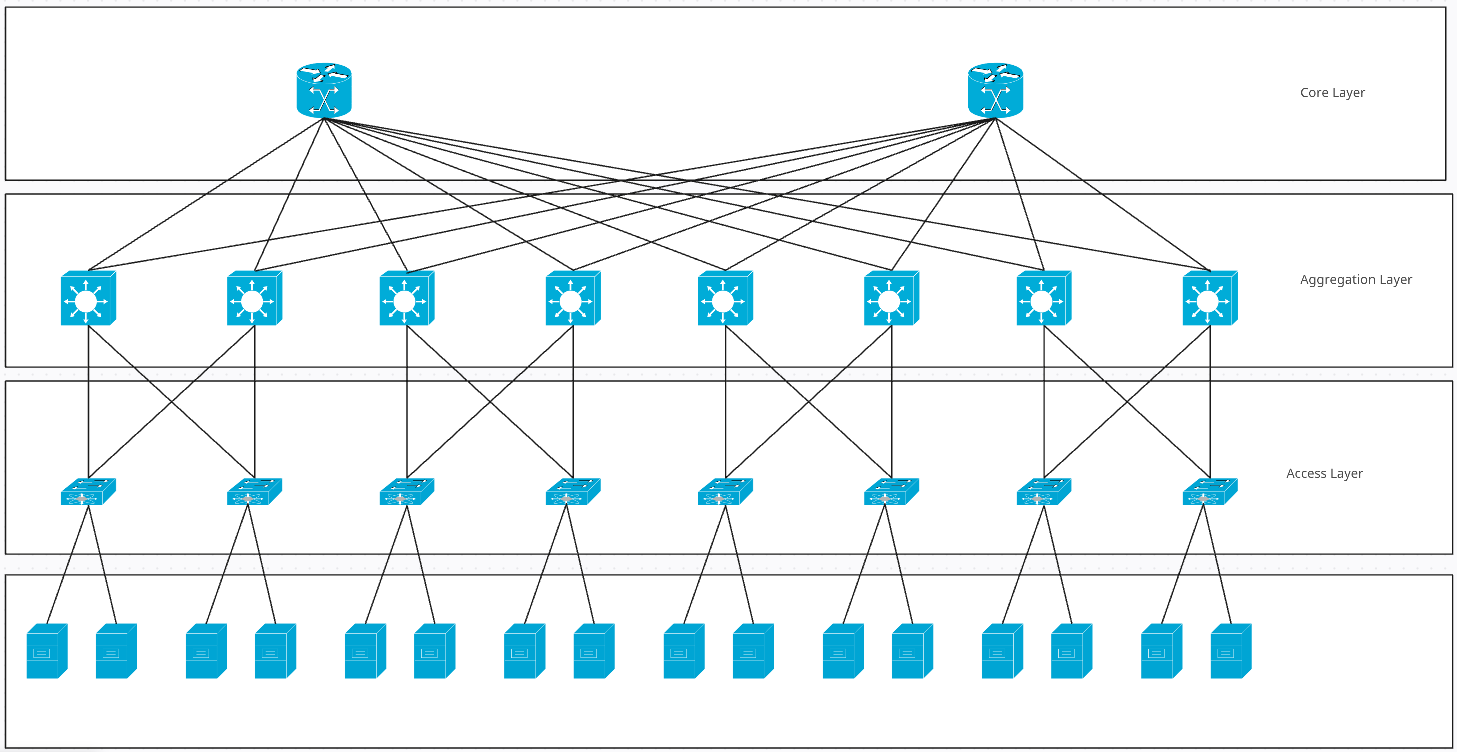
\includegraphics[width=0.85\textwidth]{images/exampletopo.png}
    \caption{Enterprise network hierarchy core, distribution, access layers}
    \label{fig:Enterprise-network-hierarchy}
\end{figure}



\subsection{Discovery Protocols: \gls{snmp} and \gls{lldp} }
The automated discovery of the topology of the network involves the use of established management protocols such as the Simple Network Management Protocol (\gls{snmp}) and the Link Layer Discovery Protocol (\gls{lldp} ). \gls{snmp} uses a management protocol involving management systems querying the individual nodes for information from the Management Information Bases ( \gls{mib} s), which store information about the equipment (ex: neighbors, IP addresses, performance and statuses ...etc) \cite{Automatic20Discovery20of20Physical20Topology20in20Ethernet20Networks}. While the \gls{snmp} plays a critical role in collecting information about the devices, \gls{lldp}  functions at the data-link layer to allow devices to announce  their identity and capabilities  \cite{Using-Link-Layer-Discovery-Protocol-in-Multivendor-Networks} 

\begin{figure}[H]
    \centering
    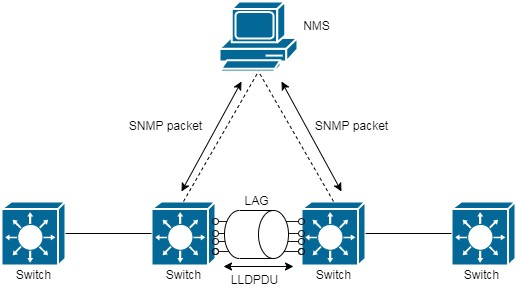
\includegraphics[width=0.85\textwidth]{images/lldp-lacp.jpg}
    \caption{\gls{snmp} - \gls{lldp}  Discovery}
    \label{fig:\gls{snmp}lldp}
\end{figure}



\section{Artificial Intelligence and Network Automation}
\subsection{Large Language Models (\gls{llm} s)}
\gls{llm} s are deep learning models based on the transformer architecture, which learns the intricate relationship between tokens through self-attention mechanisms. These models are pretrained using a huge corpus of text data including languages, coding, network RFCs, and technical writing, making them adept at language understanding and generation capabilities \cite{GN5-2-White-Paper_Gen-AI-in-Network-Management} ,\cite{Large_Language_Models_for_Networking}.In the context of network operations, \gls{llm} s represent a shift from predictive/discriminative approaches toward generative systems capable of contextual reasoning \cite{GN5-2-White-Paper_Gen-AI-in-Network-Management}.

\begin{figure}[H]
    \centering
    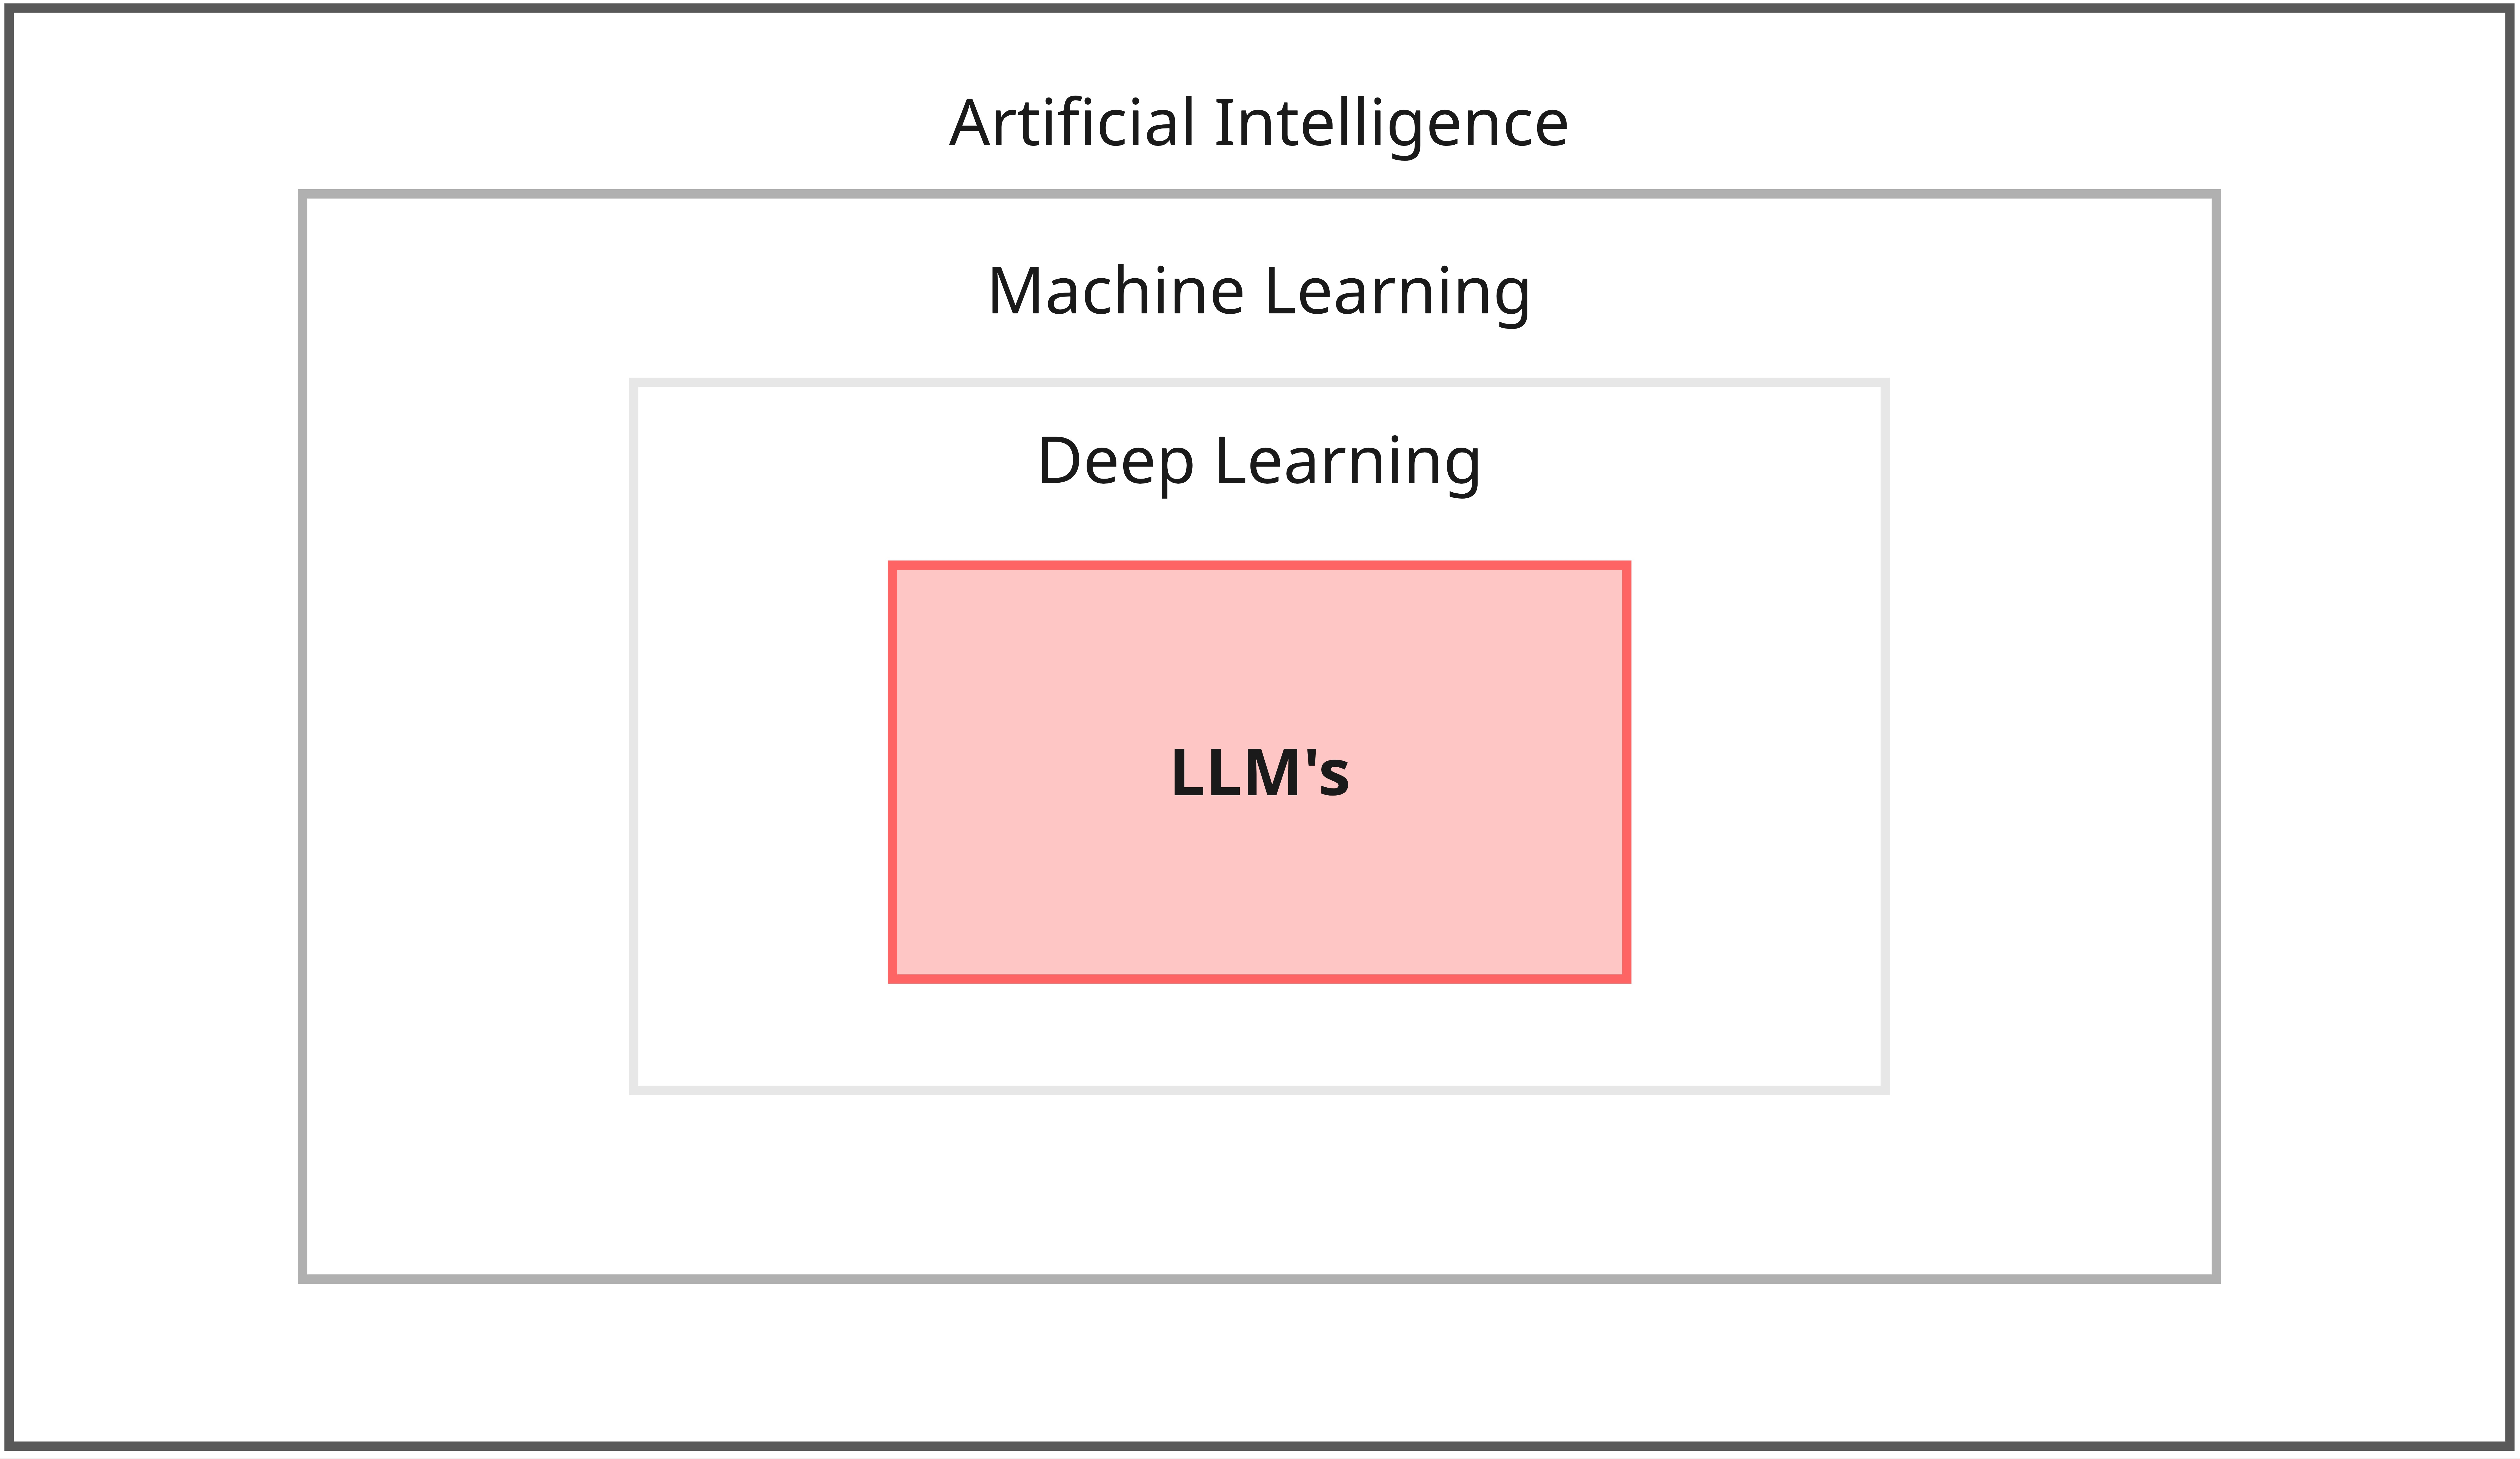
\includegraphics[width=0.85\textwidth]{images/llmvsdl.jpg}
    \caption{\gls{ai}-> ML -> DL -> \gls{llm} }
    \label{fig:LLMVSDSL}
\end{figure}


\subsection{AI Agents}
An \gls{ai}agent can be described as an intelligent agent, in which the \gls{llm}  forms the main component within a perception-reasoning-tool with an execution loop used to achieve autonomous tasks.  \cite{AgentOps}
\begin{figure}[H]
    \centering
    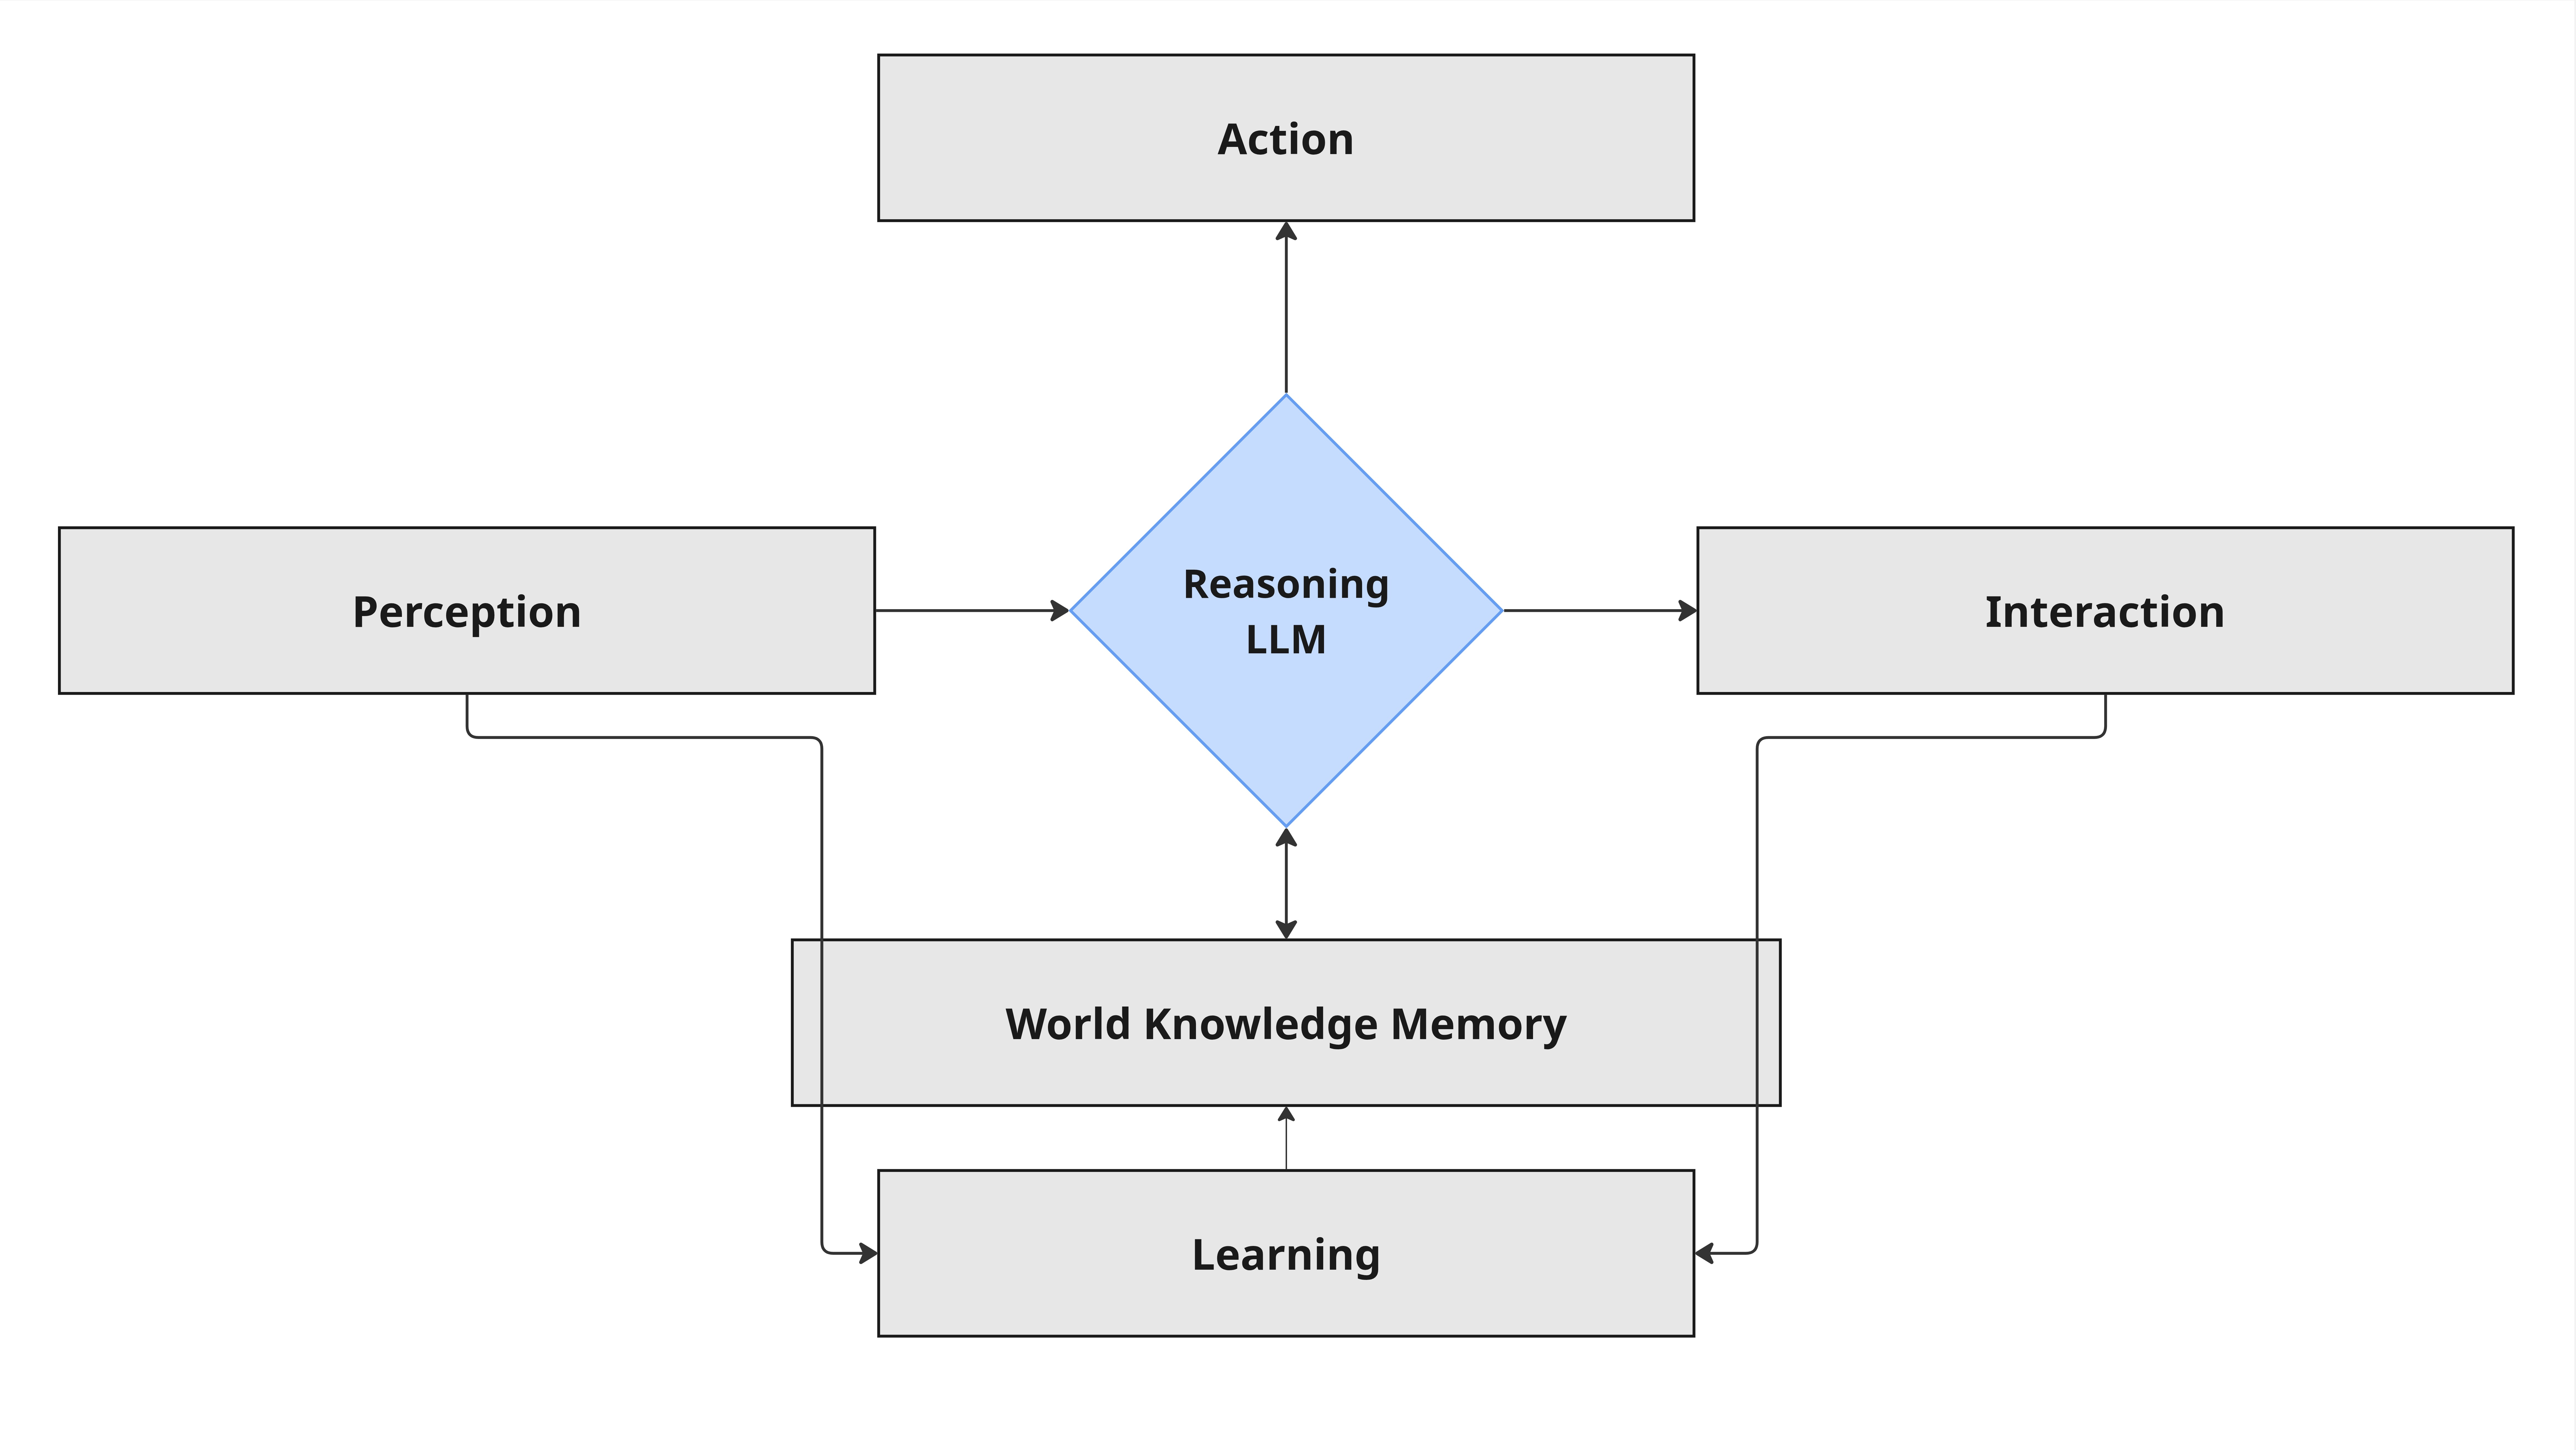
\includegraphics[width=0.85\textwidth]{images/Aiagent.jpg}
    \caption{Agentic Loop}
    \label{fig:Aiagentloop}
\end{figure}


\subsection{Intent-Based Networking (\gls{ibn}) and Zero-Touch Management}
Intent-based networking (\gls{ibn}) is a higher-level networking approach that leverages and extends Software Defiend Networking SDN principles by adding closed-loop automation, enabling the translation of high-level business goals into low-level network configurations \cite{A_Survey_on_Intent-Based_Networking}. By focusing more on what is meant in terms of the desired result rather than how a network function should be technically implemented, \gls{ibn} removes the intricacies of infrastructure \cite{A_Survey_on_Intent-Based_Networking, ZTM}.

A closed-loop architecture entails four basic elements 
\begin{itemize}
  \item \textbf{Intent Profiling} : The First step of \gls{ibn} is intent capturing
  \item \textbf{Translation} : The Second step is Translating the intent into network policies
  \item \textbf{Resolution / Activation} : The 3rd Step is provision of resources by activating intents
  \item \textbf{Assurance} :  Verification to ensure intent consistency
\end{itemize}
\cite{A_Survey_on_Intent-Based_Networking}.

\begin{figure}[H]
    \centering
    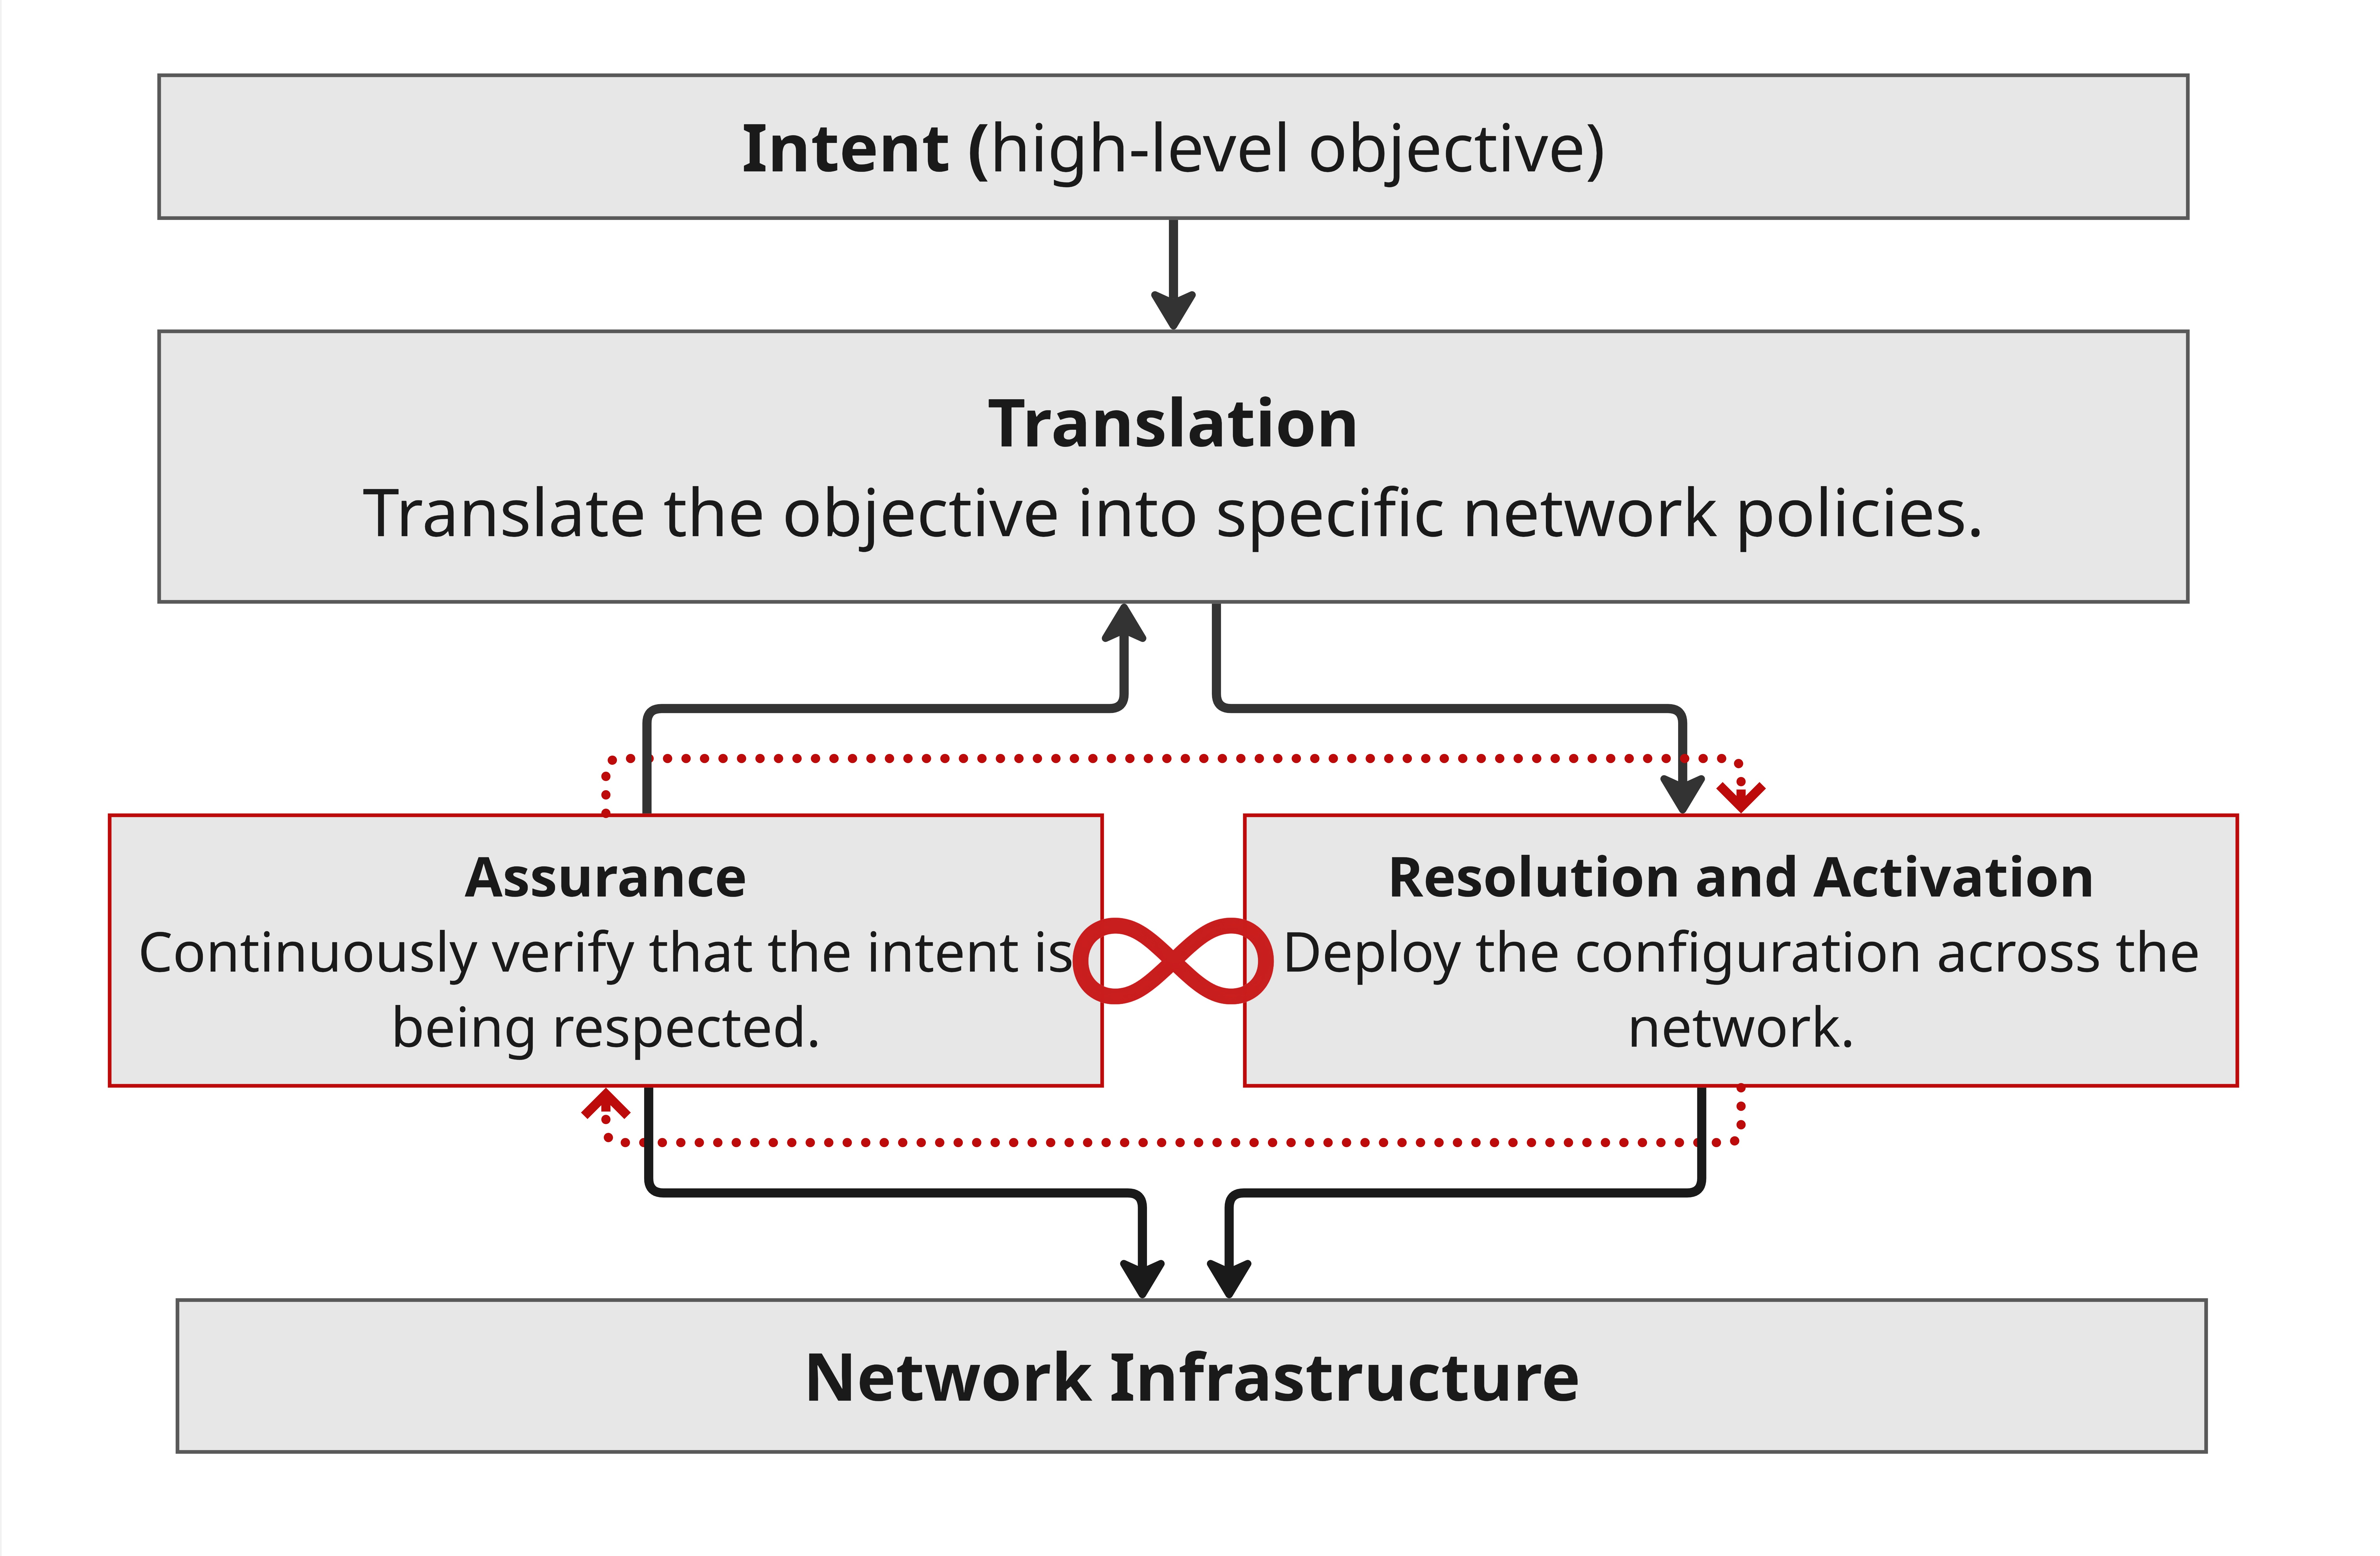
\includegraphics[width=0.85\textwidth]{images/ibnloop.jpg}
    \caption{Intent-Based Networking Loop}
    \label{fig:ibnloop}
\end{figure}


\subsection{Retrieval-Augmented Generation ( \gls{rag} )}
 \gls{rag}  refers to a framework or a technique that enhances the trustworthiness of large language models (\gls{llm} s) through the integration of external knowledge during the interaction with the \gls{llm}  \cite{AGENTIC-RETRIEVAL-AUGMENTED-GENERATION-A-SURVEY-ON-AGENTIC-RAG}. The  \gls{rag}  process typically involves several key stages:
\begin{enumerate}
    \item mapping the query provided by the user into a vector format using an embedding technique
    \item conducting a vector search on the set of indexed external documents
    \item retrieving the k-most relevant pieces of evidence and appending these pieces of evidence to the \gls{llm}  prompt.
\end{enumerate}
\cite{A-Survey-on-Retrieval-Augmented-Text-Generation-for-Large-Language-Models}

\begin{figure}[H]
    \centering
    
\includegraphics[width=0.80\textwidth]{images/RagArchituture.jpg}
    \caption{Retrieval-Augmented Generation Architecture  \gls{rag} }
    \label{fig:ragarch}
\end{figure}


In the context of networking operations, the key purpose of  \gls{rag}  is to minimize the chances of "\gls{hallucination}s," whereby \gls{llm} s generate plausible but inaccurate output \cite{AGENTIC-RETRIEVAL-AUGMENTED-GENERATION-A-SURVEY-ON-AGENTIC-RAG, A-Survey-on-Retrieval-Augmented-Text-Generation-for-Large-Language-Models}. and In networking, even a small configuration error can cause an outage that may cost a company millions of dollars.

\subsection{Model Context Protocol (MCP)}
Model Context Protocol (MCP) is an open standard that was developed by Anthropic in 2024 as a universal connector between any \gls{llm}  and any external source of data and tooling. Called the "USB-C for AI"\gls{mcp}  establishes a communication standard allowing agents to connect to various resources and datasets or even other agents \cite{Model-Context-Protocol-MCP-:-Landscape-Security-Threats-and-Future-Research-Directions}.

\begin{figure}[H]
    \centering
    
\includegraphics[width=0.85\textwidth]{images/mcp.jpg}
    \caption{\gls{llm}  w Model Context Protocol VS \gls{api}}
    \label{fig:mcpvsapi}
\end{figure}

\chapter{State of the Art: \gls{ai}for Network Operations}
\section{Current Approaches to LLM-Driven Network Operations}
The use of Large Language Models (\gls{llm} s) in the area of network operations has led to the shift from legacy, manually operated workflows to automated, intent-based approaches. An example of such approach includes LLM-NetCFG, where a locally run Zephyr 7B parameters \gls{llm}  translates natural language intents to router configurations in a private manner while achieving a high accuracy with the deterministic verification loop using "Batfish". Thus, it correctly implements high-level networking requirements, such as ACL and OSPF configuration and more \cite{ZTM}.

\begin{figure}[H]
    \centering
    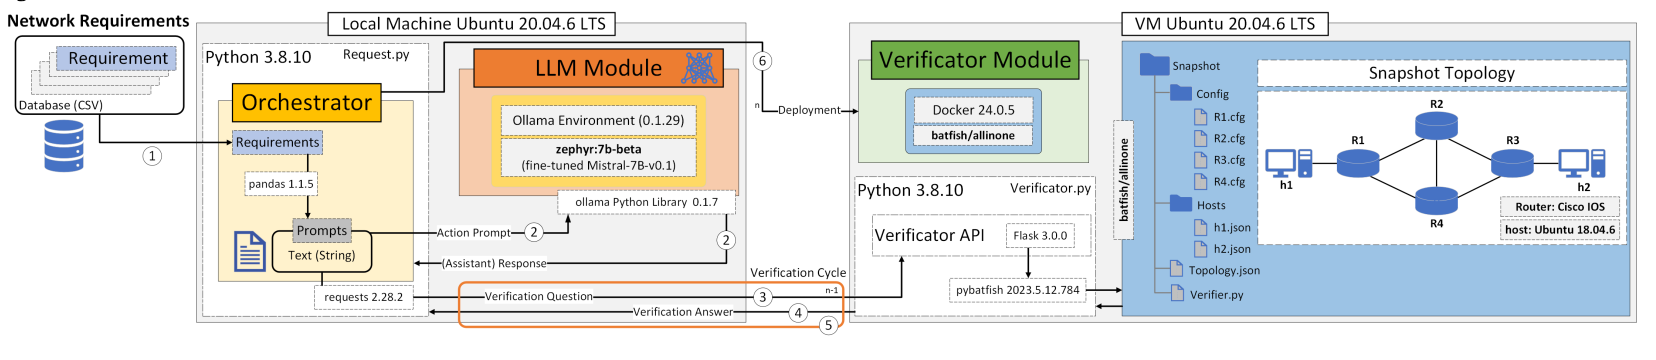
\includegraphics[width=0.85\textwidth]{images/LLMNETCFG.png}
    \caption{Example : LLM-NetCFG Structure \cite{ZTM}}
    \label{fig:LLM-NetCFG}
\end{figure}

Going further, NetLLM considers the role that Large Language Models can play in the domain of networking in the context of their utilization as general purpose foundation models applicable for solving various networking problems, including bitrate adaptation and job scheduling. Using the multi modal encoders, NetLLM maps non-textual inputs into the \gls{llm}  token space and shows a high performance gain compared to specialized algorithms \cite{NetLLM}.

\begin{figure}[H]
    \centering
    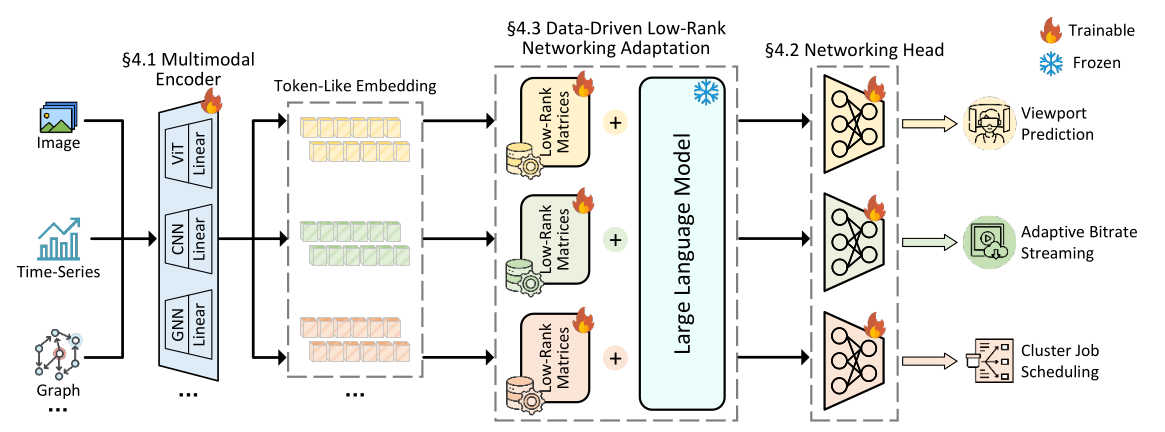
\includegraphics[width=0.85\textwidth]{images/netllm.png}
    \caption{NetLLM Structure \cite{NetLLM}}
    \label{fig:NetLLM}
\end{figure}
For end-to-end life cycle management, NetIntent  uses a form of agentic automation technology that translates intention, activates the process, and ensures continuous assurance in software-defined networking (SDN). Dynamic re-prompting and feedback are used in the technology to automatically resolve any conflicts in the flows, hence providing consistent and error-free deployment on Open Daylight and ONOS controllers\cite{NetIntent}.

\begin{figure}[H]
    \centering
    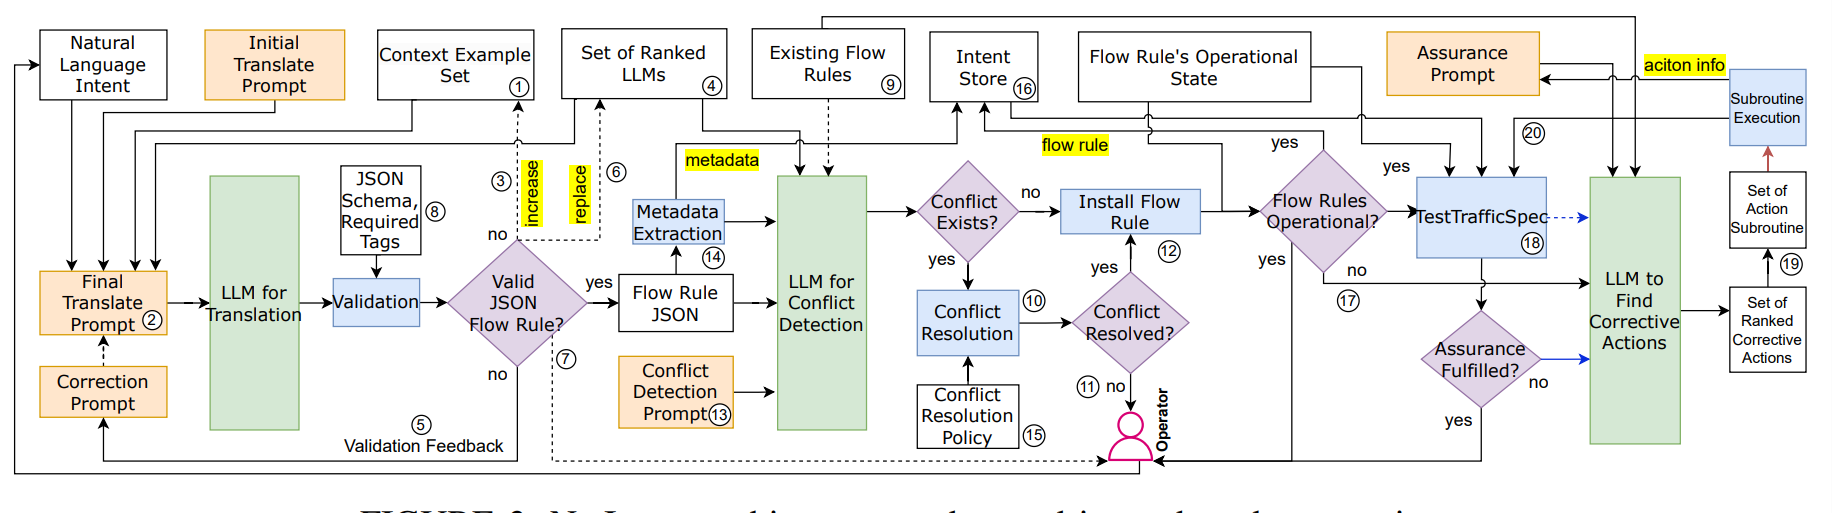
\includegraphics[width=0.85\textwidth]{images/netintent.png}
    \caption{NetIntent Structure \cite{NetIntent}}
    \label{fig:Netintent}
\end{figure}
Moreover, there is another framework called Aether that combines generative agentic artificial intelligence with a network digital twin (NDT) to generate a highly accurate virtual sandbox to validate network changes made by the agent . The framework uses special-purpose agents to test changes before production, and in actual ISP incidents, all the errors have been accurately identified within six to seven minutes \cite{Aether}.

\begin{figure}[H]
    \centering
    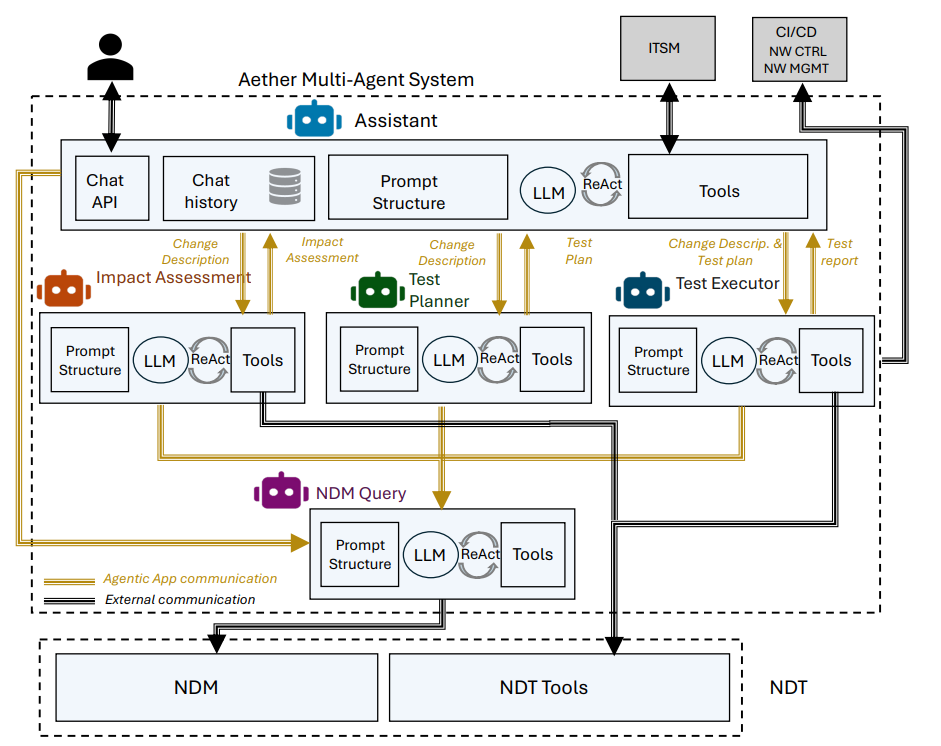
\includegraphics[width=0.85\textwidth]{images/aether.png}
    \caption{Aether Structure \cite{Aether}}
    \label{fig:aether}
\end{figure}

\section{Integrating Topology into LLMs}
The key problem associated with the development of self-driving networks involves the bridging of the network context in order to provide Large Language Models (\gls{llm} s) with sufficient knowledge about the corresponding network infrastructure  \cite{INTEGRATION-OF-LIVE-NETWORK-KNOWLEDGE-GRAPHS-WITH-RAG-FOR-ENHANCE}.

In order to tackle this problem, there are many proposed methods to ground \gls{ai}reasoning on the actual connectivity, thus making sure that the output remains true and accurate.

\subsection{Topology as text}
The first and most obvious way to establish a connection between \gls{llm} s and network context is to serialize topology information into human readable formats that can further be fed into the prompt for \gls{ai}systems. As a result, the process involves the transformation of the network infrastructure into natural language representation  \cite{Large-Language-Models-for-Networking:-Workflow}.

Researchers usually prefer using structured languages such as XML, YAML, YANG, or JSON as they provide high flexibility while transmitting and storing information also an advantage is these structured languages use fewer tokens than free text.\cite{yang}.

\begin{figure}[H]
\begin{verbatim}
module network-topology {
  container topology {
    list node {
      key "id";
      leaf id   { type string; }
      leaf role { type string; }
    }

    list link {
      key "id";
      leaf id     { type string; }
      leaf source { type string; }
      leaf dest   { type string; }
    }
  }
}
\end{verbatim}
\caption{Example \gls{topology} serialized as YANG.}
\end{figure}

However when representing network structure in the form of sequential text or structured languages like XML and JSON, multi-dimensional graph dependencies are simplified to sequential data, hence losing non-canonical dependencies that are required for path-aware inference \cite{Graph2text}.

\subsection{Topology as Image}
Researchers also have explored vision-language models like GPT-4 Vision and LLaVA in explaining the network diagrams generated by the emulator as well as the manually drawn diagrams. In this regard, an example of the approach can be the GeNet framework. Such an approach is consistent with the workflow of various industries where whiteboards are used throughout network engineering  \cite{GeNET}.


\begin{figure}[H]
    \centering
    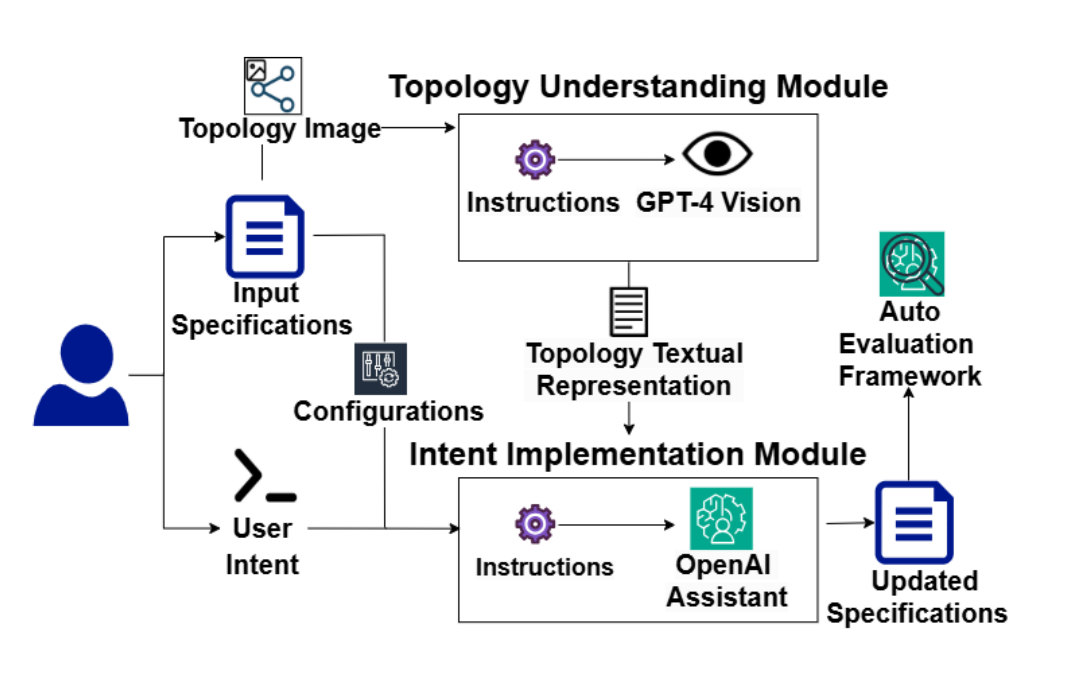
\includegraphics[width=0.85\textwidth]{images/genet.png}
    \caption{GeNet Structure \cite{GeNET}}
    \label{fig:Genet}
\end{figure}

However, GeNet's topology extraction accuracy is significantly influenced by input quality (Image), with hand-drawn sketches and messy layouts results in accuracy. Furthermore, missing structural details like interface labels hinder the model's ability to precisely interpret and map the network's connectivity \cite{GeNET}.

\subsection{Topology as a Knowledge Graph}
The Knowledge Graph (KG) framework offers the strongest method to ensure that there is topological awareness by considering the devices as discrete nodes while the logical and/or physical connections between those devices(network equipment) form edges(Connections between network equipment ex: peer,connected ...etc). The operational information such as the state of interfaces, speed, and VLAN configurations are then considered the properties attached to the entities, making it a network source of truth \cite{INTEGRATION-OF-LIVE-NETWORK-KNOWLEDGE-GRAPHS-WITH-RAG-FOR-ENHANCE}


\subsection{Graph as Text}
"Graph2text" \gls{topology} serialization aims to transform the physical infrastructures into language-based explanations, adjacency lists, or XML/JSON format, ready to be used as inputs for prompt injections. This approach is mainly employed due to the ease of adoption, lack of requirements for infrastructure, and the ability of the Large Language Model (\gls{llm} ) to understand the texts \cite{Graph2text}


\begin{figure}[H]
    \centering
    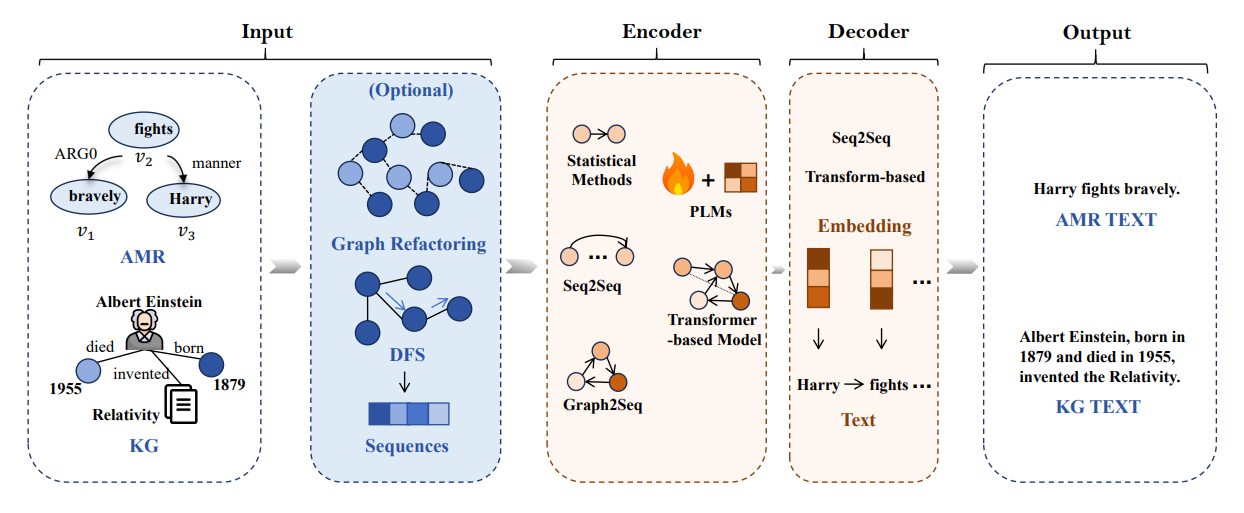
\includegraphics[width=0.85\textwidth]{images/graph2text.png}
    \caption{Graph2Text  \gls{textualization}  method.  \cite{Graph2text}}
    \label{fig:graph2text}
\end{figure}

However, such an approach is limited to smaller-sized networks because as soon as infrastructures involving roughly 1,000 devices, they exceed token capacities and context windows.

\subsection{Vector-Based  \gls{rag}  on Topology Chunks}
As an alternative solution, topology could be divided into chunks with semantic meaning (ex: individual data-center sites, security zones or DMZ's ...etc), which could be stored in a vector database for similarity searches \cite{INTEGRATION-OF-LIVE-NETWORK-KNOWLEDGE-GRAPHS-WITH-RAG-FOR-ENHANCE}.
Although this improves retrieval efficiency over full injection but still this method is giving the \gls{llm}  chunks that are irrelevant to the problem increasing the \gls{hallucination} also the reliance on flat cosine similarity remains a fundamental barrier to structural reasoning .


\subsection{Knowledge Graph RAG}

By converting natural language questions into graph traversals and retrieving relevant subgraphs, Knowledge Graph RAG (\gls{graphrag}) circumvents these issues, as it enables multi-hop reasoning necessary for thematic evolution and indirect relationships between network entities giving more presise context to the \gls{llm}  for reasoning \cite{GraphRAG, Understanding-GraphRAG}.

\begin{figure}[H]
    \centering
    
\includegraphics[width=0.85\textwidth]{images/kgrag.jpg}
    \caption{High Level Knowledge \gls{graphrag}}
    \label{fig:kgrag}
\end{figure}





\section{The Current Gap and Limitations}
In spite of all of the recent progress made in \gls{grounding} and visual \gls{grounding} tasks, one particular challenge remains unmet: there is no known solution that allows incorporating a constantly changing topographical dataset together with the capability of a corresponding \gls{ai}model to utilize on-demand depth-dependent network subgraphs. Such lack of solution leads to the constant issue of "\gls{topologicalblindness}" that limits agents in either their constant dependence on out-of-date context or inability to follow complex dependencies in multi-hop reasoning tasks. It is exactly this functionality need that gives grounds to introduce the  \gls{trag}  and  \gls{tmcp}  mechanism duo presented in the next chapter.


\chapter{Proposed Approach: Integrating \gls{topology} Graph into \gls{llm} s}
\section{Conceptual Framework:  \gls{trag}  paired with  \gls{tmcp} }
The limitations highlighted within the previous chapter, primarily referred to as "\gls{topologicalblindness}" call for a shift from an inefficient, text-oriented retrieval process to an efficient dual mechanism \gls{grounding} paradigm. This paper introduces a conceptual framework integrating both aspects to provide a complete structure understanding for the \gls{ai}agent, including Topology Knowledge Graph Retrieval-Augmented Generation ( \gls{trag} ), and an \gls{mcp} -based Topology Graph Tool ( \gls{tmcp} ).

While KG-RAG focuses on retrieving information in the first step by dividing the topology graph into relevant chunks in order to anchor the \gls{ai}agent’s prompt in real structural truth, the  \gls{tmcp}  tool empowers the \gls{ai}agent with on-demand access to the topology through its reasoning cycle.

\begin{figure}[H]
    \centering
    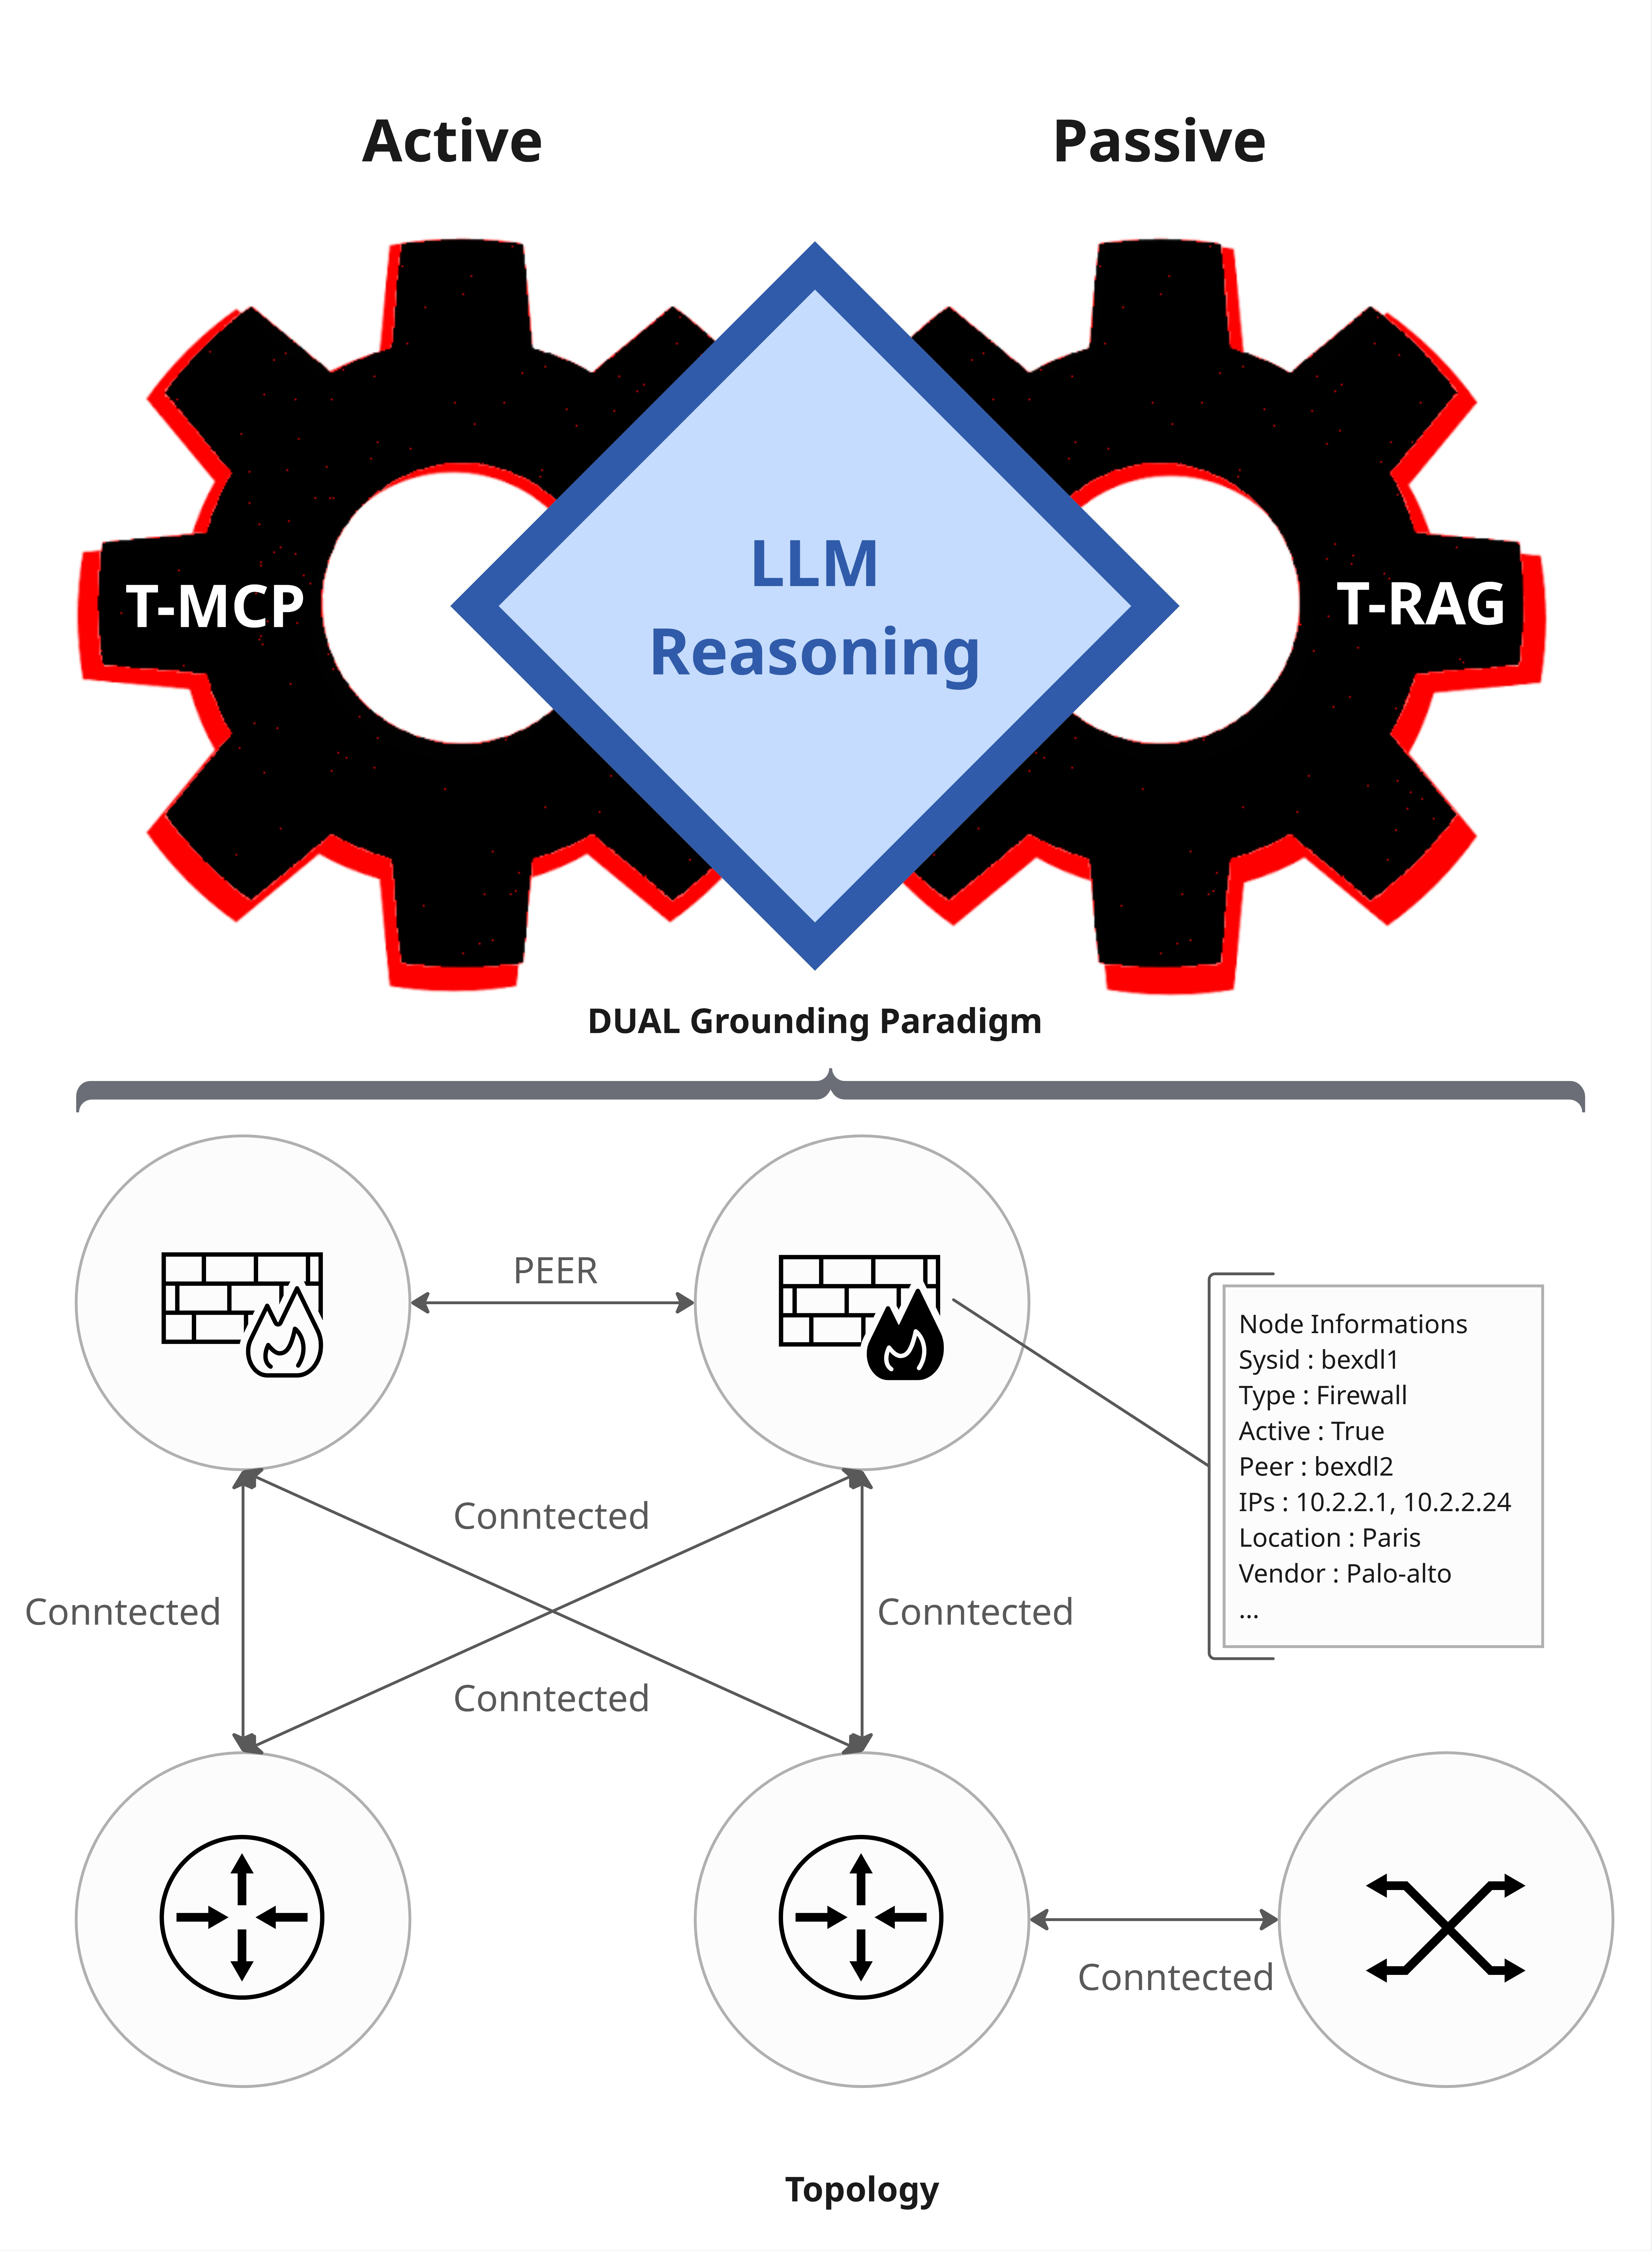
\includegraphics[width=0.6\textwidth]{images/DUALGROUNDING.jpg}
    \caption{ \gls{trag}  paired with  \gls{tmcp} }
    \label{fig:dualgrounding}
\end{figure}
This conceptual combination ensures that the \gls{ai}assistant stays aware of everything that happens in Task execution at all stages of the process .  \gls{trag}  provides a context-based starting point through retrieval of subgraphs that are relevant to the user's request, whereas  \gls{tmcp}  allows the agent to operate as a Topology Navigator by making directed requests via hostnames or IPs , and indirectly confirming dependencies when planning.



 
\section{Automatic Network Discovery and \gls{kg} Construction}
In order to build the source of truth for \gls{AINetOps}, we start with automatic discovery workflow that converts heterogeneous physical and logical interconnections into a machine-readable graph. For this purpose, we implement a two-step recursive approach that ensures error-free reflection of the production network in the resulting  \gls{neo4j}  database without introducing errors due to manual input of the data.

The first step includes implementation of a discovery engine in the form of a Python script, which performs multiple requests starting from a certain seed node. By using \gls{snmp} with \gls{lldp} , we perform poll of the devices for management information contained in standardized  \gls{mib} s. Using \gls{lldp}  advertisements, our script discovers attributes of each node along with the list of its neighbors, thus identifying direct physical interconnections regardless of vendor-specific interfaces. 

\begin{table}[H]
\centering
\caption{\gls{snmp}  \gls{mib}   \gls{oid} s utilized by the discovery script.}
\label{tab:\gls{snmp}-oids}
\small
\begin{tabular}{ll}
\toprule
\textbf{Category /  \gls{oid}  Name} & \textbf{ \gls{oid} } \\
\midrule
\multicolumn{2}{l}{\textit{System}} \\
OID\_SYS\_DESCR    & 1.3.6.1.2.1.1.1.0 \\
OID\_SYS\_NAME     & 1.3.6.1.2.1.1.5.0 \\
OID\_SYS\_UPTIME   & 1.3.6.1.2.1.1.3.0 \\
OID\_SYS\_LOCATION & 1.3.6.1.2.1.1.6.0 \\
\midrule
\multicolumn{2}{l}{\textit{IP}} \\
OID\_IP\_ADDR\_TABLE & 1.3.6.1.2.1.4.20.1.1 \\
OID\_IP\_FORWARDING  & 1.3.6.1.2.1.4.1.0 \\
\midrule
\multicolumn{2}{l}{\textit{Interfaces}} \\
OID\_IF\_INDEX       & 1.3.6.1.2.1.2.2.1.1 \\
OID\_IF\_DESCR       & 1.3.6.1.2.1.2.2.1.2 \\
OID\_IF\_TYPE        & 1.3.6.1.2.1.2.2.1.3 \\
OID\_IF\_MTU         & 1.3.6.1.2.1.2.2.1.4 \\
OID\_IF\_SPEED       & 1.3.6.1.2.1.2.2.1.5 \\
OID\_IF\_ADMIN\_STATUS & 1.3.6.1.2.1.2.2.1.7 \\
OID\_IF\_OPER\_STATUS  & 1.3.6.1.2.1.2.2.1.8 \\
OID\_IF\_HIGH\_SPEED   & 1.3.6.1.31.1.1.1.15 \\
\midrule
\multicolumn{2}{l}{\textit{\gls{lldp} }} \\
OID\_LLDP\_REM\_TABLE      & 1.0.8802.1.1.2.1.4.1.1 \\
OID\_LLDP\_REM\_CHASSIS\_ID & 1.0.8802.1.1.2.1.4.1.1.5 \\
OID\_LLDP\_REM\_PORT\_DESC  & 1.0.8802.1.1.2.1.4.1.1.8 \\
OID\_LLDP\_REM\_SYS\_NAME   & 1.0.8802.1.1.2.1.4.1.1.9 \\
OID\_LLDP\_REM\_SYS\_DESC   & 1.0.8802.1.1.2.1.4.1.1.10 \\
OID\_LLDP\_REM\_MAN\_ADDR   & 1.0.8802.1.1.2.1.4.2 \\
\midrule
\multicolumn{2}{l}{\textit{Physical Inventory}} \\
OID\_ENT\_PHYSICAL\_DESCR  & 1.3.6.1.2.1.47.1.1.1.1.2 \\
OID\_ENT\_PHYSICAL\_MODEL  & 1.3.6.1.2.1.47.1.1.1.1.13 \\
OID\_ENT\_PHYSICAL\_SERIAL & 1.3.6.1.2.1.47.1.1.1.1.11 \\
\bottomrule
\end{tabular}
\end{table}

The script works recursively, so when one neighbor is discovered, we automatically make the same query to this node, and continue doing so until there is no more neighbors are left in the network to discover.


\begin{figure}[H]
    \centering
    \includegraphics[width=0.85\textwidth]{images/\gls{snmp}loop.jpg}
    \caption{Network Discovery loop}
    \label{fig:Discovery}
\end{figure}
In the second stage, a population script ingests the JSON output to instantiate the nodes and edges within the  \gls{neo4j}  graph database.

\begin{table}[H]
\centering
\caption{Edge relationship types in the  \gls{neo4j}  topology graph.}
\label{tab:edge-types} 
\small
\begin{tabular}{p{4cm} p{9cm}}
\toprule
\textbf{Edge Type} & \textbf{Meaning} \\
\midrule
CONNECTED, LAYER2 & Physical or inferred layer-2 link between devices \\
UPLINK, DOWNLINK & Hierarchical access-to-distribution or distribution-to-core links \\
PEER & Logical adjacency (BGP, OSPF, HSRP peers) \\
TRUNK, VLAN\_MEMBER & VLAN-carrying or VLAN membership relationships \\
MANAGED & Management-plane relationship between device and  \gls{nms}  \\
HIGH\_AVAILABILITY & HA pair relationship (firewall, load balancer) \\
FIBER, COPPER, WIRELESS & Physical medium type \\
\bottomrule
\end{tabular}
\end{table}

\section{Topology as a  \gls{rag} : The  \gls{trag}  Pipeline}

The  \gls{trag}  pipeline is based on a retrieval-oriented \gls{grounding} process where the context of the language model (\gls{llm} ) is automatically supplemented with validated topological data before any reasoning takes place. First, the term extraction phase starts: the natural-language request of the user is matched with regular expression which detects alphanumeric sequences including hyphens and dots, i.e. a usual notation of device hostnames and IP addresses, except a hand-curated stop-word list of typical networking terms which are unlikely to be used as device names. The extracted candidates are then sorted according to length (more specific terms are longer) and limited to six candidates, out of which the four most specific ones are sent to  \gls{neo4j} .



Then each of the terms is searched among three properties of nodes: hostname, description and location with the use of case-insensitive substring matching of  \gls{cypher}  query. For each matched device, the pipeline immediately fetches its outgoing edges via the \texttt{list\_edges} function, retrieving the one-hop neighbourhood with all physical and logical links, port identifiers, bandwidth values, and VLAN assignments. To prevent the saturation of the context window, there is a limitation of up to ten devices and up to fifteen edges per device being injected.

Finally, the obtained subgraph is serialized into concise text representation similar to YANG, instead of verbose JSON or XML. There is a reason for such an approach: the YANG-like format is machine readable and is represented with a small number of tokens while being still clear enough for the \gls{llm}  to understand. An example of output block is as follows:

\begin{figure}[H]
\begin{verbatim}
network-topology { 
  device iotlab {
    type server; status active;
    ips "10.48.255.24";
    location "TestLab rack-02";
    vendor Generic;
    link CONNECTED -> sw-access01 { 
        src Gi0; dst Gi1/0/12; bw 1G; 
    }
  }
  device sw-access01 {
    type switch; status active;
    ips "10.48.255.1";
    vendor Cisco;
    link UPLINK -> core-sw01 { 
        src Gi1/0/1; dst Gi2/0/1; bw 10G; 
    }
  }
}
\end{verbatim}
\caption{Example  \gls{trag}  YANG-style context block injected into the 
\gls{llm}  prompt for a query about \texttt{iotlab}.}
\label{fig:yang-context}
\end{figure}

This block is added to the system context of the \gls{llm}  before its reasoning starts to guarantee that every answer the agent generates will be grounded in the factual physical and logical realities of the network and not the probabilistic prior knowledge of the model.

\begin{figure}[H]
    \centering
    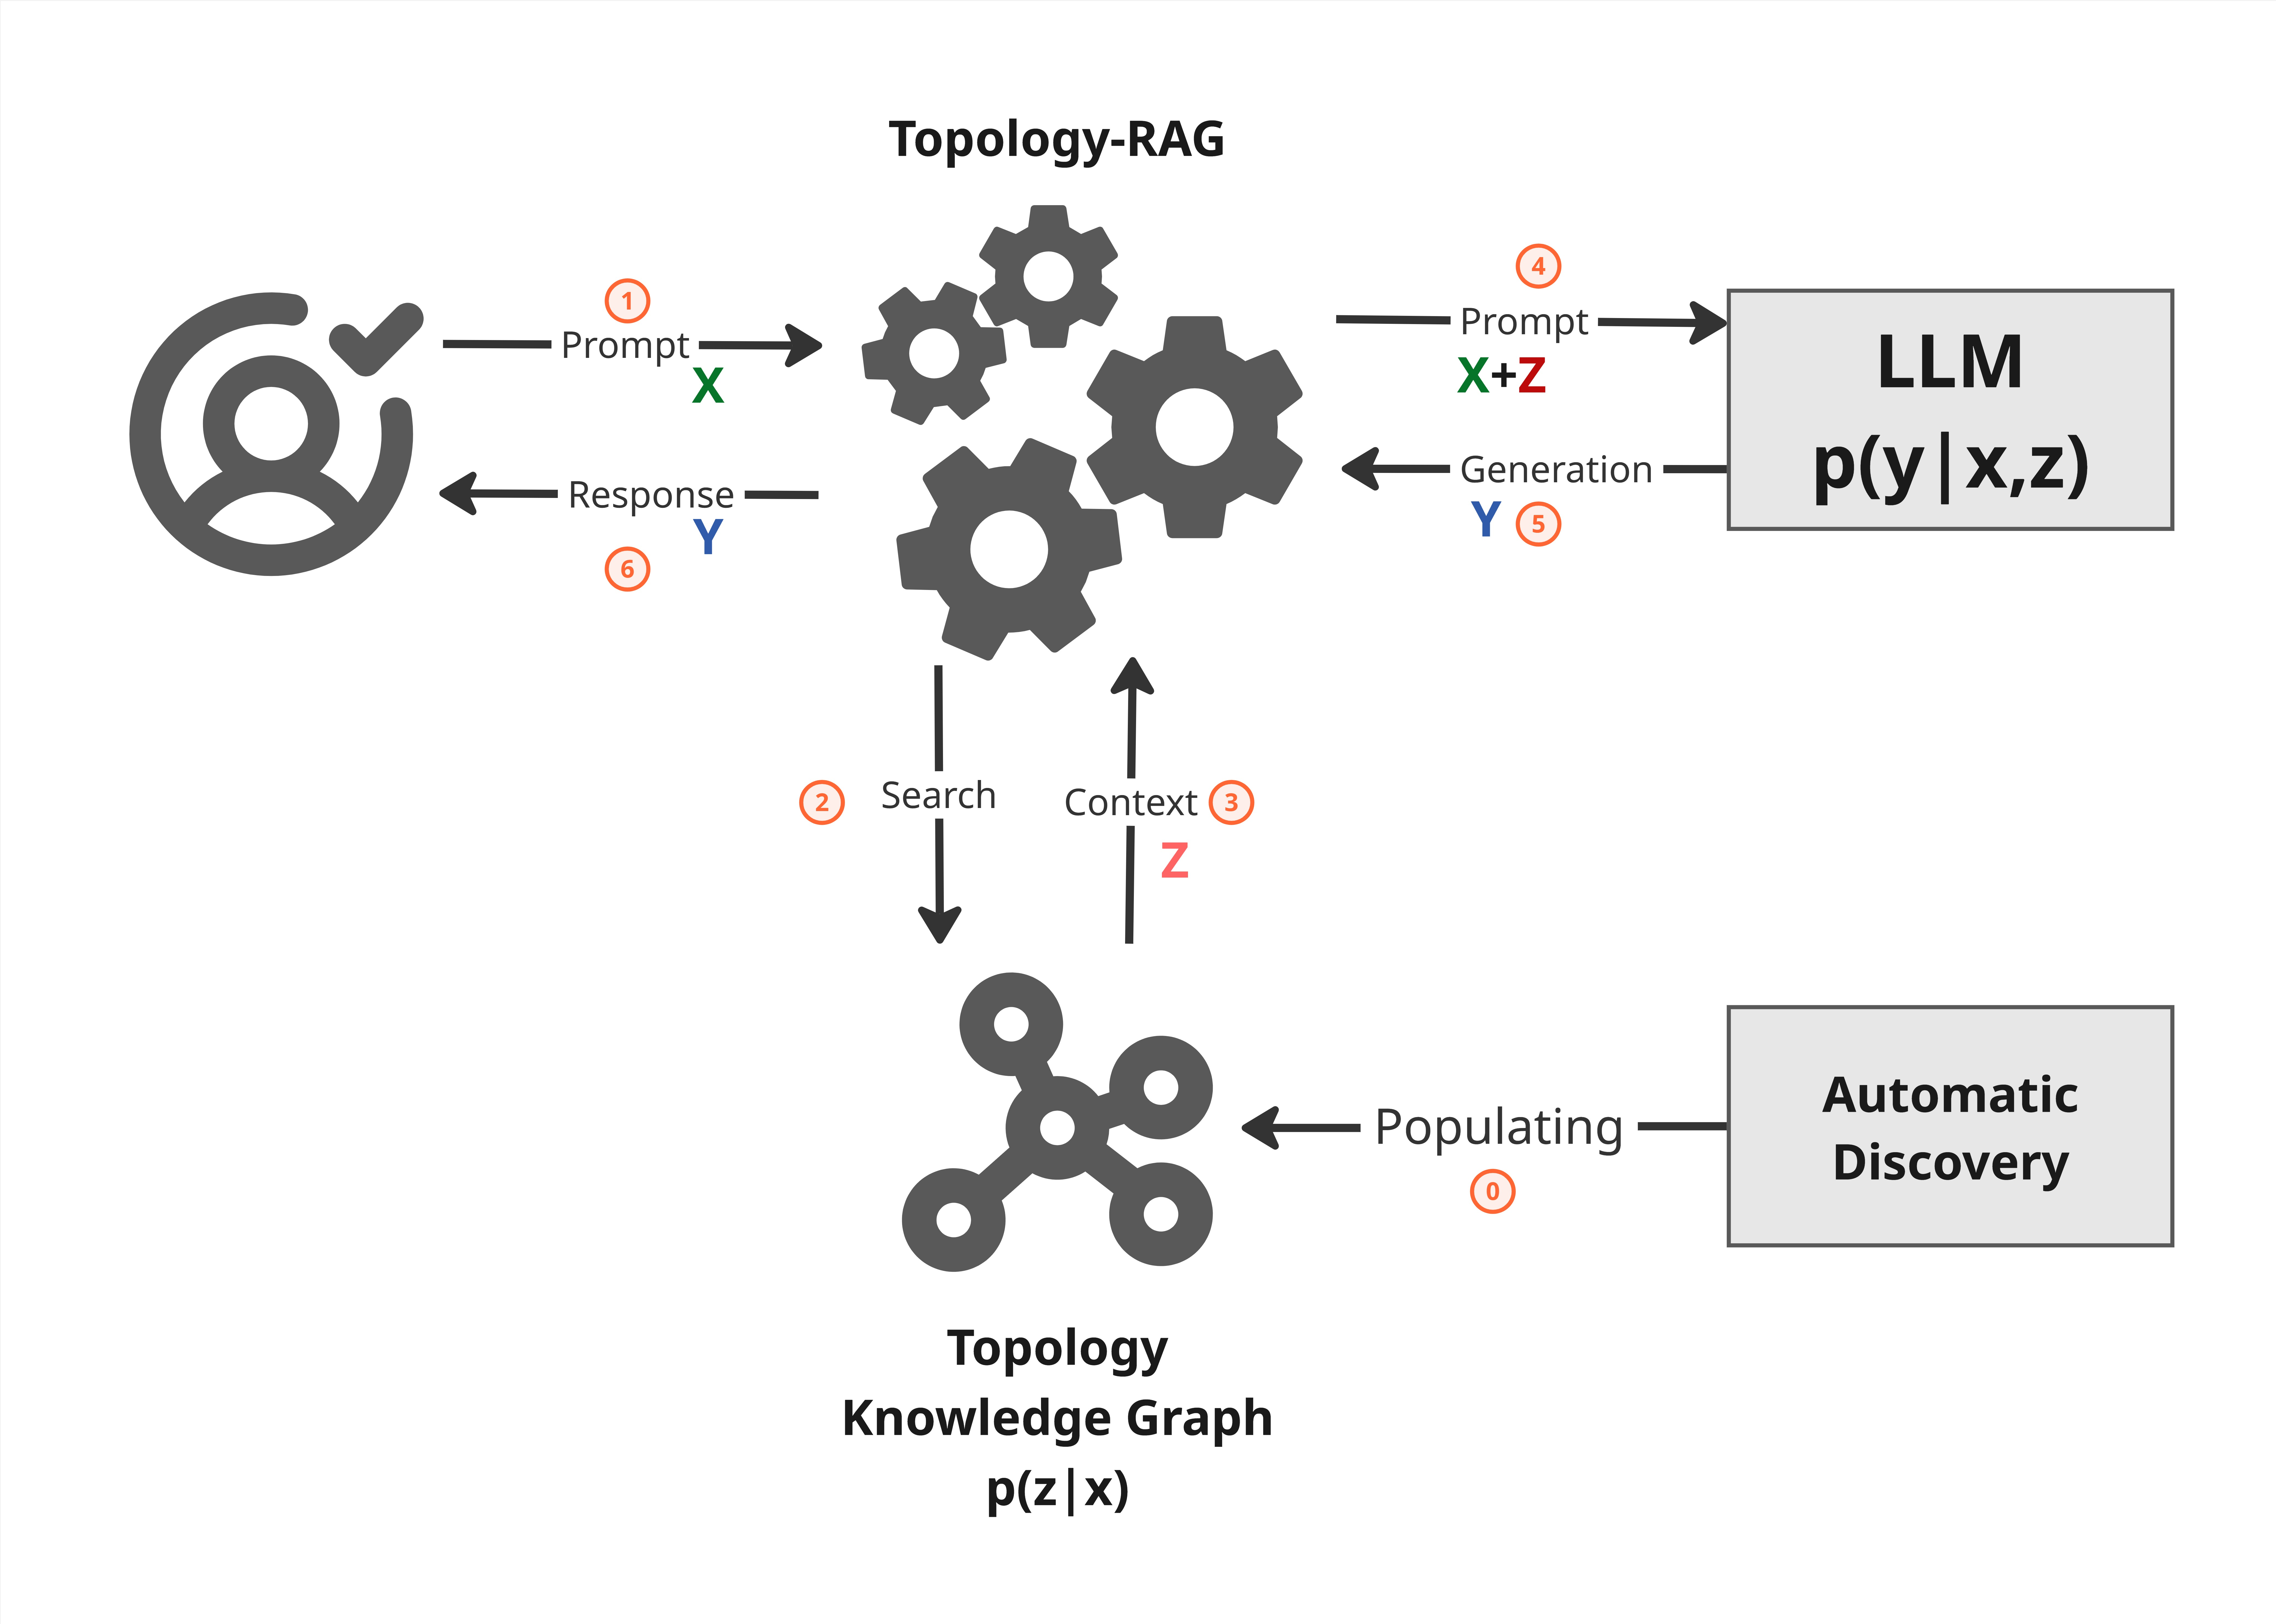
\includegraphics[width=0.85\textwidth]{images/trag.jpg}
    \caption{ \gls{trag}  pipeline}
    \label{fig:trag}
\end{figure}



\section{Topology as a Tool: Dynamic Retrieval via \gls{mcp}  ( \gls{tmcp} )}

Although  \gls{trag}  grounds the agent during prompt construction,  \gls{tmcp}  extends the topology access capability of the agent to a dynamic feature where the topology is presented to the agent as a set of on-demand tools through the direct Python-to- \gls{neo4j}  interface in the \gls{mcp}  layer. Instead of pre-loading a snapshot of a subgraph, the agent independently decides during its reasoning process when the structural information is needed and sends a request to one of the tools with a particular device identifier.


Four different tools are provided by the  \gls{tmcp}  interface, each one representing a different topological query pattern:

\begin{itemize}
    \item The \texttt{get\_topology} tool performs \textbf{BFS subgraph traversal} starting from a named device and configurable parameter of a limited depth from 1 to 10 hops. In case the APOC graph library is available, the tool uses the \texttt{path.subgraphAll} procedure; otherwise, the variable-length  \gls{cypher}  path match is used.
    \item The \texttt{get\_node} tool retrieves the property set of a single device by hostname.
    \item The \texttt{search\_nodes} tool searches any indexed property for a substring in a case-insensitive manner; hence, it enables the agent to find either partial name or IP fragment in the network graph.
    \item Finally, the \texttt{get\_path} tool calculates the \textbf{shortest path} between two named devices by  \gls{cypher}  procedure \texttt{shortestPath()} and returns the entire hop chain with all edge metadata.
\end{itemize}


\begin{table}[H]
\centering
\caption{ \gls{tmcp}  tools exposed to the \gls{ai}agent.}
\label{tab:tmcp-tools}
\small
\begin{tabular}{p{3cm} p{3.5cm} p{6cm}}
\toprule
\textbf{Tool} & \textbf{Parameters} & \textbf{Output} \\
\midrule
\texttt{get\_topology} & hostname, depth (1--10) & 
BFS subgraph: all nodes and edges within N hops \\[4pt]
\texttt{get\_node} & hostname & 
Full property set of a single device node \\[4pt]
\texttt{search\_nodes} & query, field & 
List of devices matching a substring in the given field \\[4pt]
\texttt{get\_path} & source, target & 
Shortest path with all intermediate hops and edge metadata \\
\bottomrule
\end{tabular}
\end{table}

An important architectural decision was made that the execution of these tool calls would be performed as direct  calls against the  \gls{neo4j}  driver instead of the HTTP request to an intermediate \gls{mcp}  server as in the case of the incident correlation tools working against Elasticsearch. This design ensures zero network latency from the topology queries and allows making several queries per one agent reasoning cycle.

The response from each tool is serialized using the same YANG-like formatter as  \gls{trag}  to ensure consistency of the context in terms of the number of tokens whether the topology data were pre-loaded or dynamically retrieved. The returned subgraph can be further used by the agent in its reasoning process, which allows performing fully iterative navigation of the topology: first call finds the device by IP, the second its neighbors, and finally the third finds the shortest path to a certain faulty location.

\begin{figure}[H]
    \centering
    
\includegraphics[width=0.85\textwidth]{images/tmcp.jpg}
    \caption{ \gls{tmcp}  Reasoning Loop}
    \label{fig:tmcp}
\end{figure}

\newpage
\subsection{Full proposed approach workflow}
\begin{figure}[H]
    \centering
    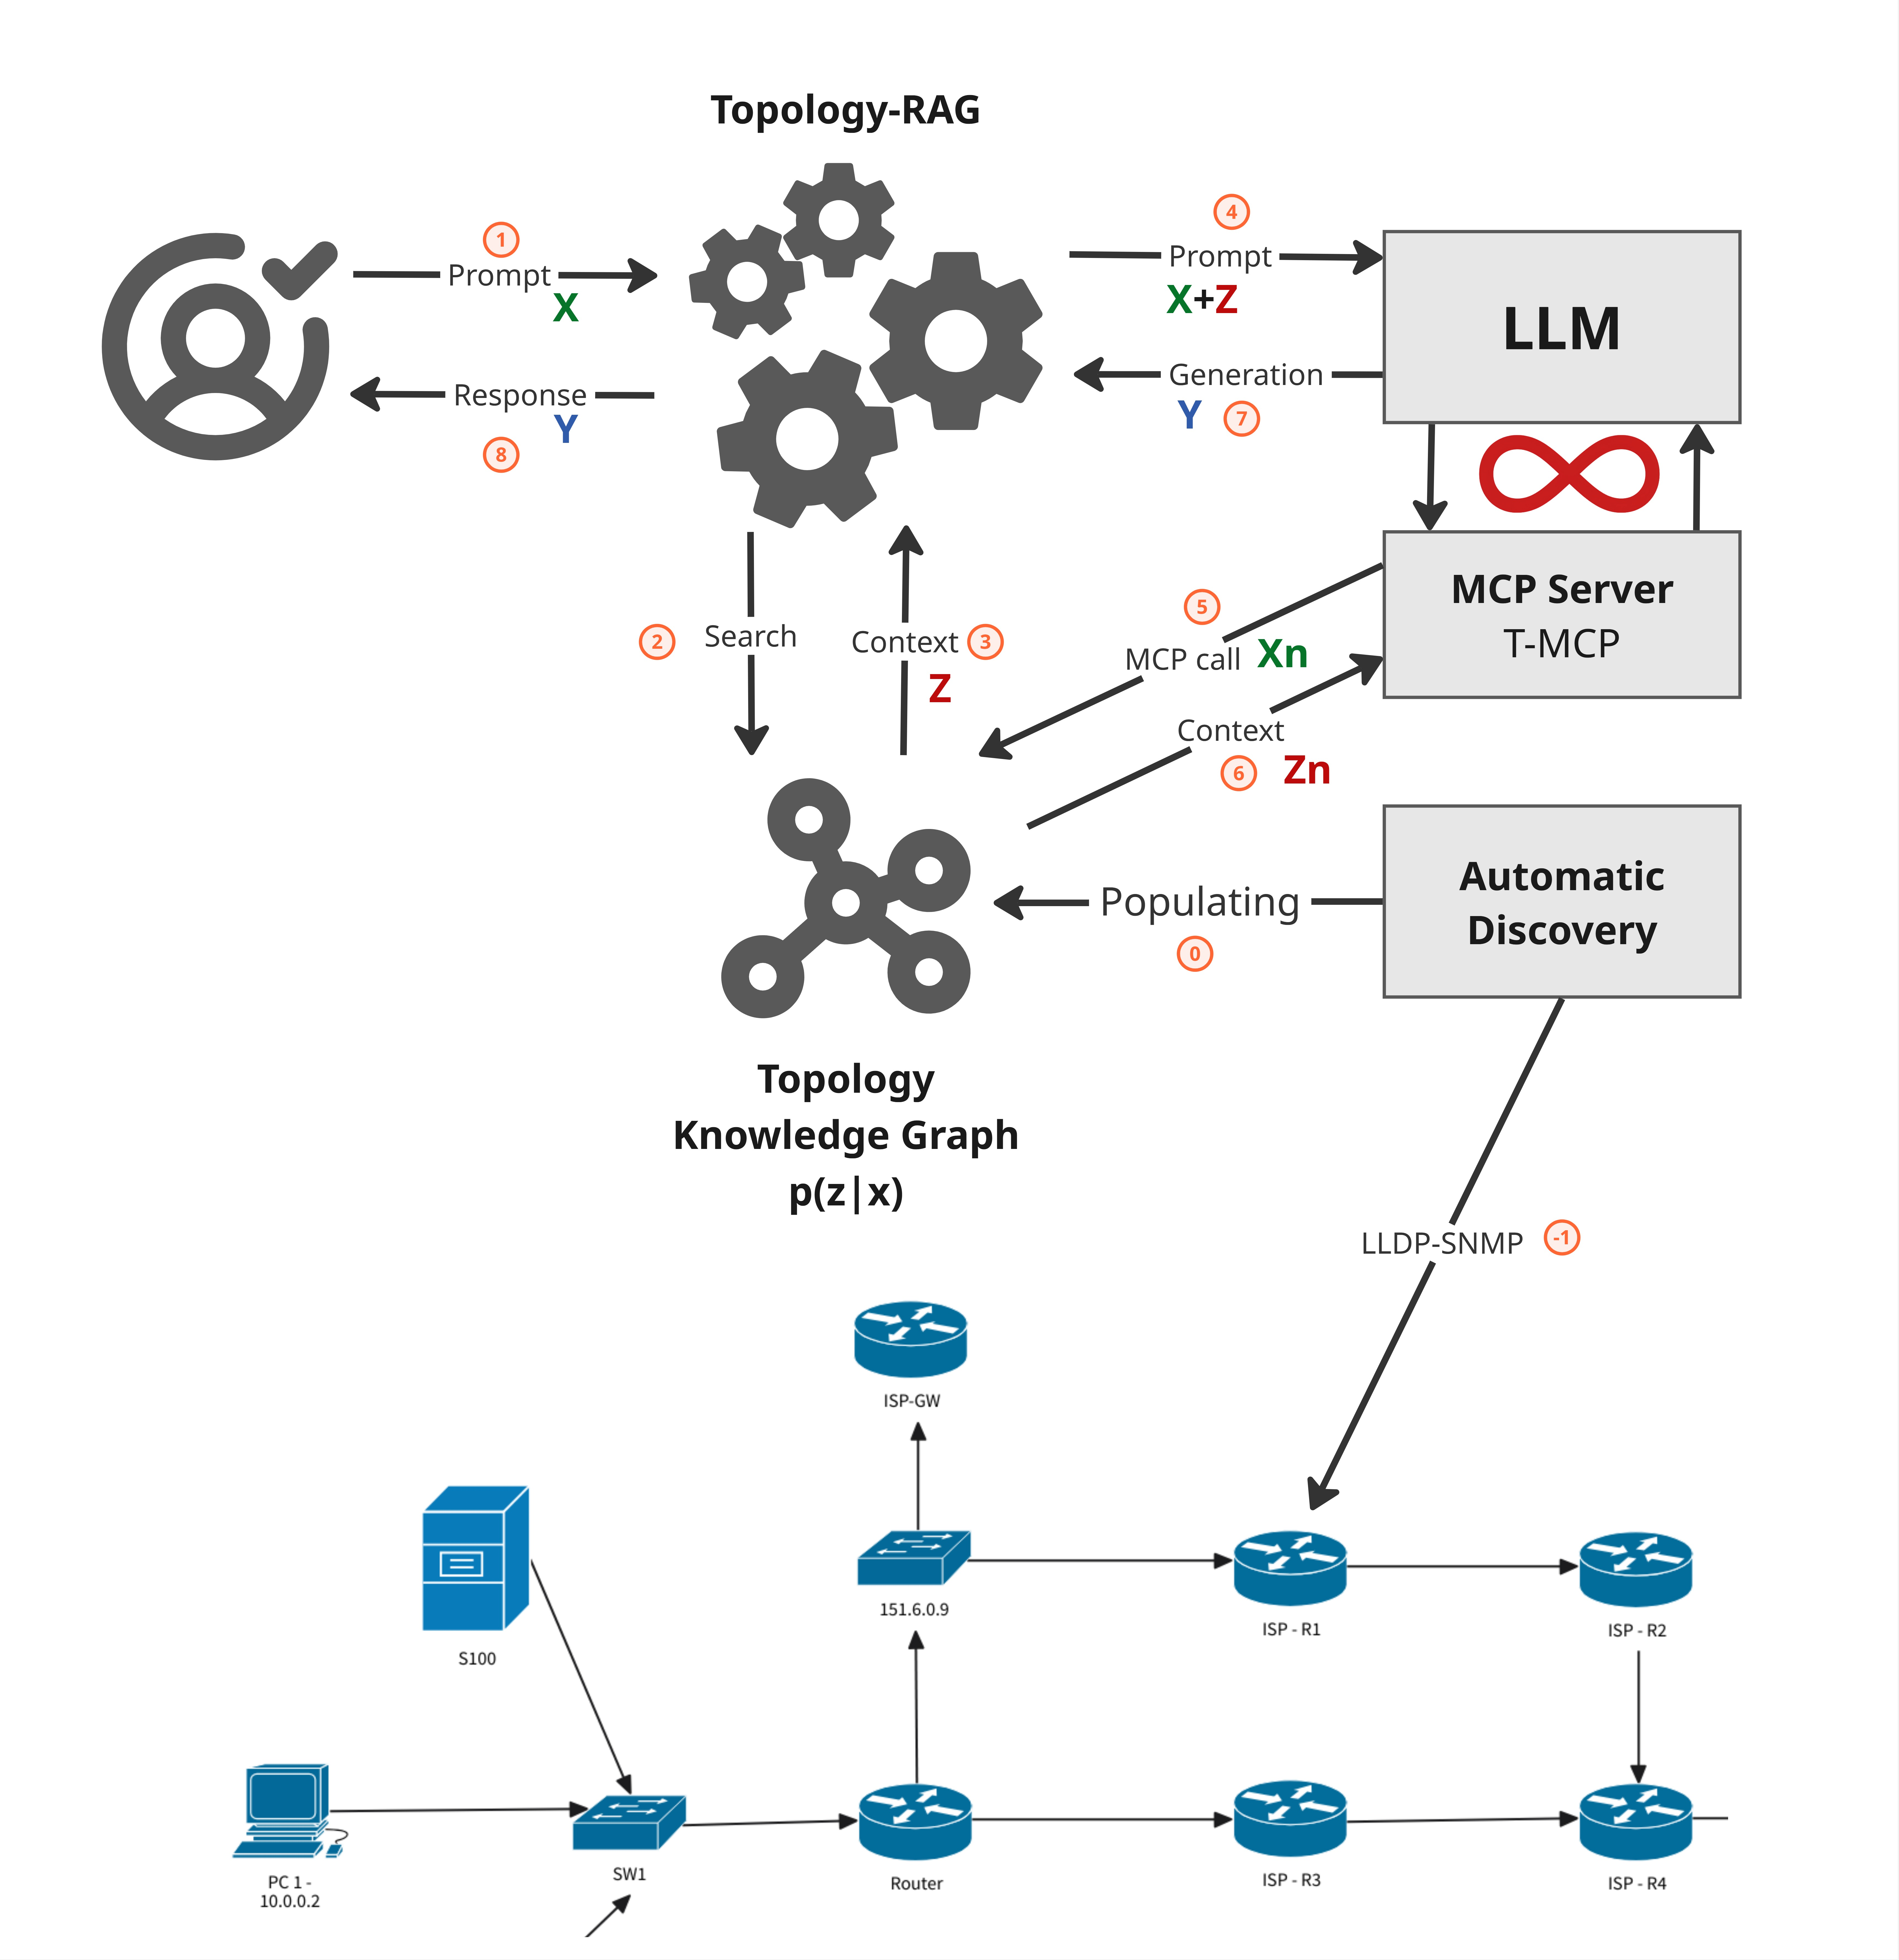
\includegraphics[width=0.9\textwidth]{images/tmcp+trag.jpg}
    \caption{Workflow: from automatic topology discovery to  \gls{trag}  and  \gls{tmcp}  grounded agent reasoning.}
    \label{fig:fullworkflow}
\end{figure}


\chapter{Evaluation and Results}

\section{Methodology and Test Scenarios}

For evaluating the performance of \gls{ai}agents influenced by topology \gls{grounding}, an experiment was carried out in a realistic Test Lab. In the process of evaluation, four different levels have been set for testing, ranging from a basic level where there is an absence of any support in the form of context, to a fourth level where the agent has been equipped with the topology tools ( \gls{tmcp}  and  \gls{trag} ).

The test environment consists of a realistic enterprise network as illustrated in Figure~\ref{fig:testlab}, including switches, a firewall,  core switch, and a wireless LAN controller interconnected across the \texttt{10.48.255.0/24} subnet.

\begin{figure}[H]
    \centering
    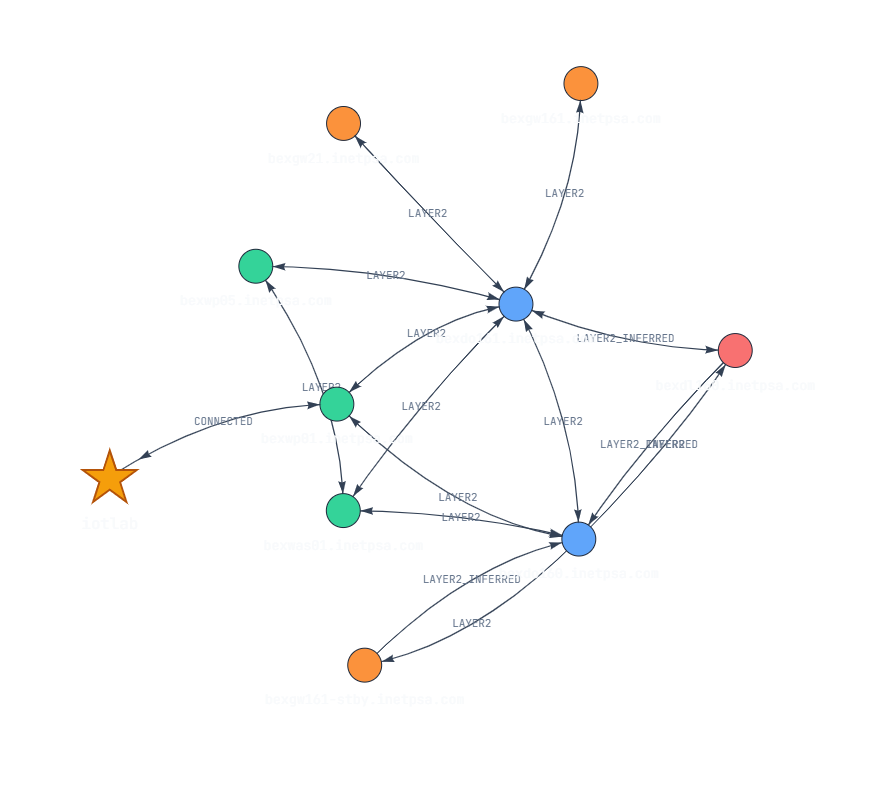
\includegraphics[width=0.85\textwidth]{images/test.png}
    \caption{Test lab architecture used for evaluation.}
    \label{fig:testlab}
\end{figure}

The fault situation was created through the physical disconnection of the link connecting the IoTLab device in the test environment hosted on iotlab.com (with an IP address of 10.48.255.24, which has a web server). Such an arrangement represents a realistic possibility for a layer-2 network problem, making the device unreachable by ping and HTTP requests.

The following command was entered into the agent for each experiment:

\begin{quote}
\textit{"A user can't connect to \texttt{iotlab} or ping it. Fix it."}
\end{quote}

The prompt was deliberately formulated in a vague manner in order to test the autonomy in diagnosing each of the conditions. In reality, when dealing with a network issue, a network engineer would follow a structured troubleshooting process: resolve the \gls{fqdn} to its IP address, identify which device the IP belongs to, check for recent firewall rule changes, trace the path to the connected switch, verify the physical link state on the relevant interface, check peer adjacency, and ultimately SSH into the upstream device to inspect the port status.

Each condition is measured across three aspects :
\begin{enumerate}
    \item  \textbf{Diagnostic Accuracy :} correct identification of the device and the source of the problem
    \item \textbf{Autonomy :} Proactive behavior of the agent or asking questions
    \item \textbf{\gls{hallucination} :} Creating non-existent facts based on the current network environment
\end{enumerate}




\section{Baseline: LLM Without Contextual Aids}
In the case of the baseline scenario, the agent operates using only its prior training without being able to consult documentation, topology information, or other diagnostic utilities. It is clear that the agent cannot make any assumptions about the specific network and therefore gives general vendor-independent advice on how to deal with the issue at hand. For example, it suggests such basic actions as checking the cable connection or even flushing the ARP cache.

Importantly, the agent is not able to determine the device on the IP address, determine what switch the device is attached to, or determine at which layer in the OSI model the problem occurs. The agent takes no automatic action or exhibits any diagnostic capability. This situation supports the fundamental limitation discussed in Chapter 3: without any underlying structure, an \gls{llm}  will be incapable of performing network functions beyond basic advice that could be given by a junior engineer.

\section{Performance with Standard Document  \gls{rag} }
When supplemented by retrieval augmented generation using document indexing ( \gls{rag} ), the agent will have access to documents in the knowledge base that provide descriptions of the test lab. As a result, there is clear improvement in terms of the agent’s performance as it can correctly identify that the subnet within which 10.48.255.0/24 belongs is the test lab subnet with switches, firewalls, core switch, and  \gls{wlc} . An example of the agent’s response is provided below:

\begin{quote}
\textit{"What should be running on \texttt{iotlab}? I can see from the documentation that \texttt{iotlab} is the test lab environment network that contains switches, firewalls, core switches, and  \gls{wlc} . Before I run diagnostic scripts, I need to confirm what device or service should be at .24. Is this affecting just one user or multiple users? Are other devices in the \texttt{10.48.255.0/24} range accessible?"}
\end{quote}

This development represents a considerable improvement. however, the agent still fails to detect what kind of device is sitting on iotlab, its significance in the topology of the network, and the switch port it is plugged into. The agent cannot perform an autonomous operation because it lacks the structure knowledge required for locating the fault. Document  \gls{rag}  contains semantic information, but it does not contain the topological information. The agent knows about the neighborhood but does not know how to move around in it.



\section{Performance with Knowledge \gls{graphrag} ( \gls{trag} )}

In the scenario where  \gls{trag}  is enabled, the first message from the agent will include a subgraph generated from the knowledge graph stored in  \gls{neo4j} , which centers around node 10.48.255.24 and its N-hop neighborhood. As a result, the quality of the diagnostic process changes right away – the agent correctly recognizes that the device is an IoT lab server, determines its \gls{fqdn} (iotlab.com), finds out about its upstream switch and identifies the physical connection between the two devices. Thanks to such information, the agent does not need to ask clarifying questions, and proceeds straight to the right part of the network and gives relevant recommendations for fixing the topology.

The agent recognizes that the device is connected to one particular switch port, checks if adjacency is created through this switch and recommends checking out the interface of the upstream device. This reasoning process is consistent with how a senior network engineer would think of resolving such a problem. There are no \gls{hallucination}s present since all the mentioned devices and connections are taken from the verified knowledge graph and not inferred probabilistically.

However,  \gls{trag}  itself is still a passive process, where the subgraph is pre-loaded when constructing the prompt, and the agent cannot make subsequent topology queries during the reasoning process.

% ─────────────────────────────────────────────────────────────────────
\section{Performance with Dynamic Topology Tooling ( \gls{tmcp} )}

 \gls{tmcp}  supplies the agent with topology information graphs to serve as an on-the-fly \gls{mcp}  tool, does not require the acquisition of a pre-fetched subgraph but rather constructs the  \gls{cypher}  query that is tailored to the agent’s reasoning process through device identifiers, like system ID, IP address, or host name.

Once the fault message is received, the first step taken by the agent is to invoke the  \gls{tmcp}  tool with the query argument 10.48.255.24. The tool retrieves the device node, its attributes, and its adjacent neighbors. Further, the agent calls another tool to find out the state of the switch port interface connected with the failed link. Once the disabled link is identified, the agent automatically runs the necessary diagnostic script available in the  \gls{nop}  automation layer without any human interaction to check the interface and suggest re-enabling the port.
\begin{figure}[H]
    \centering
    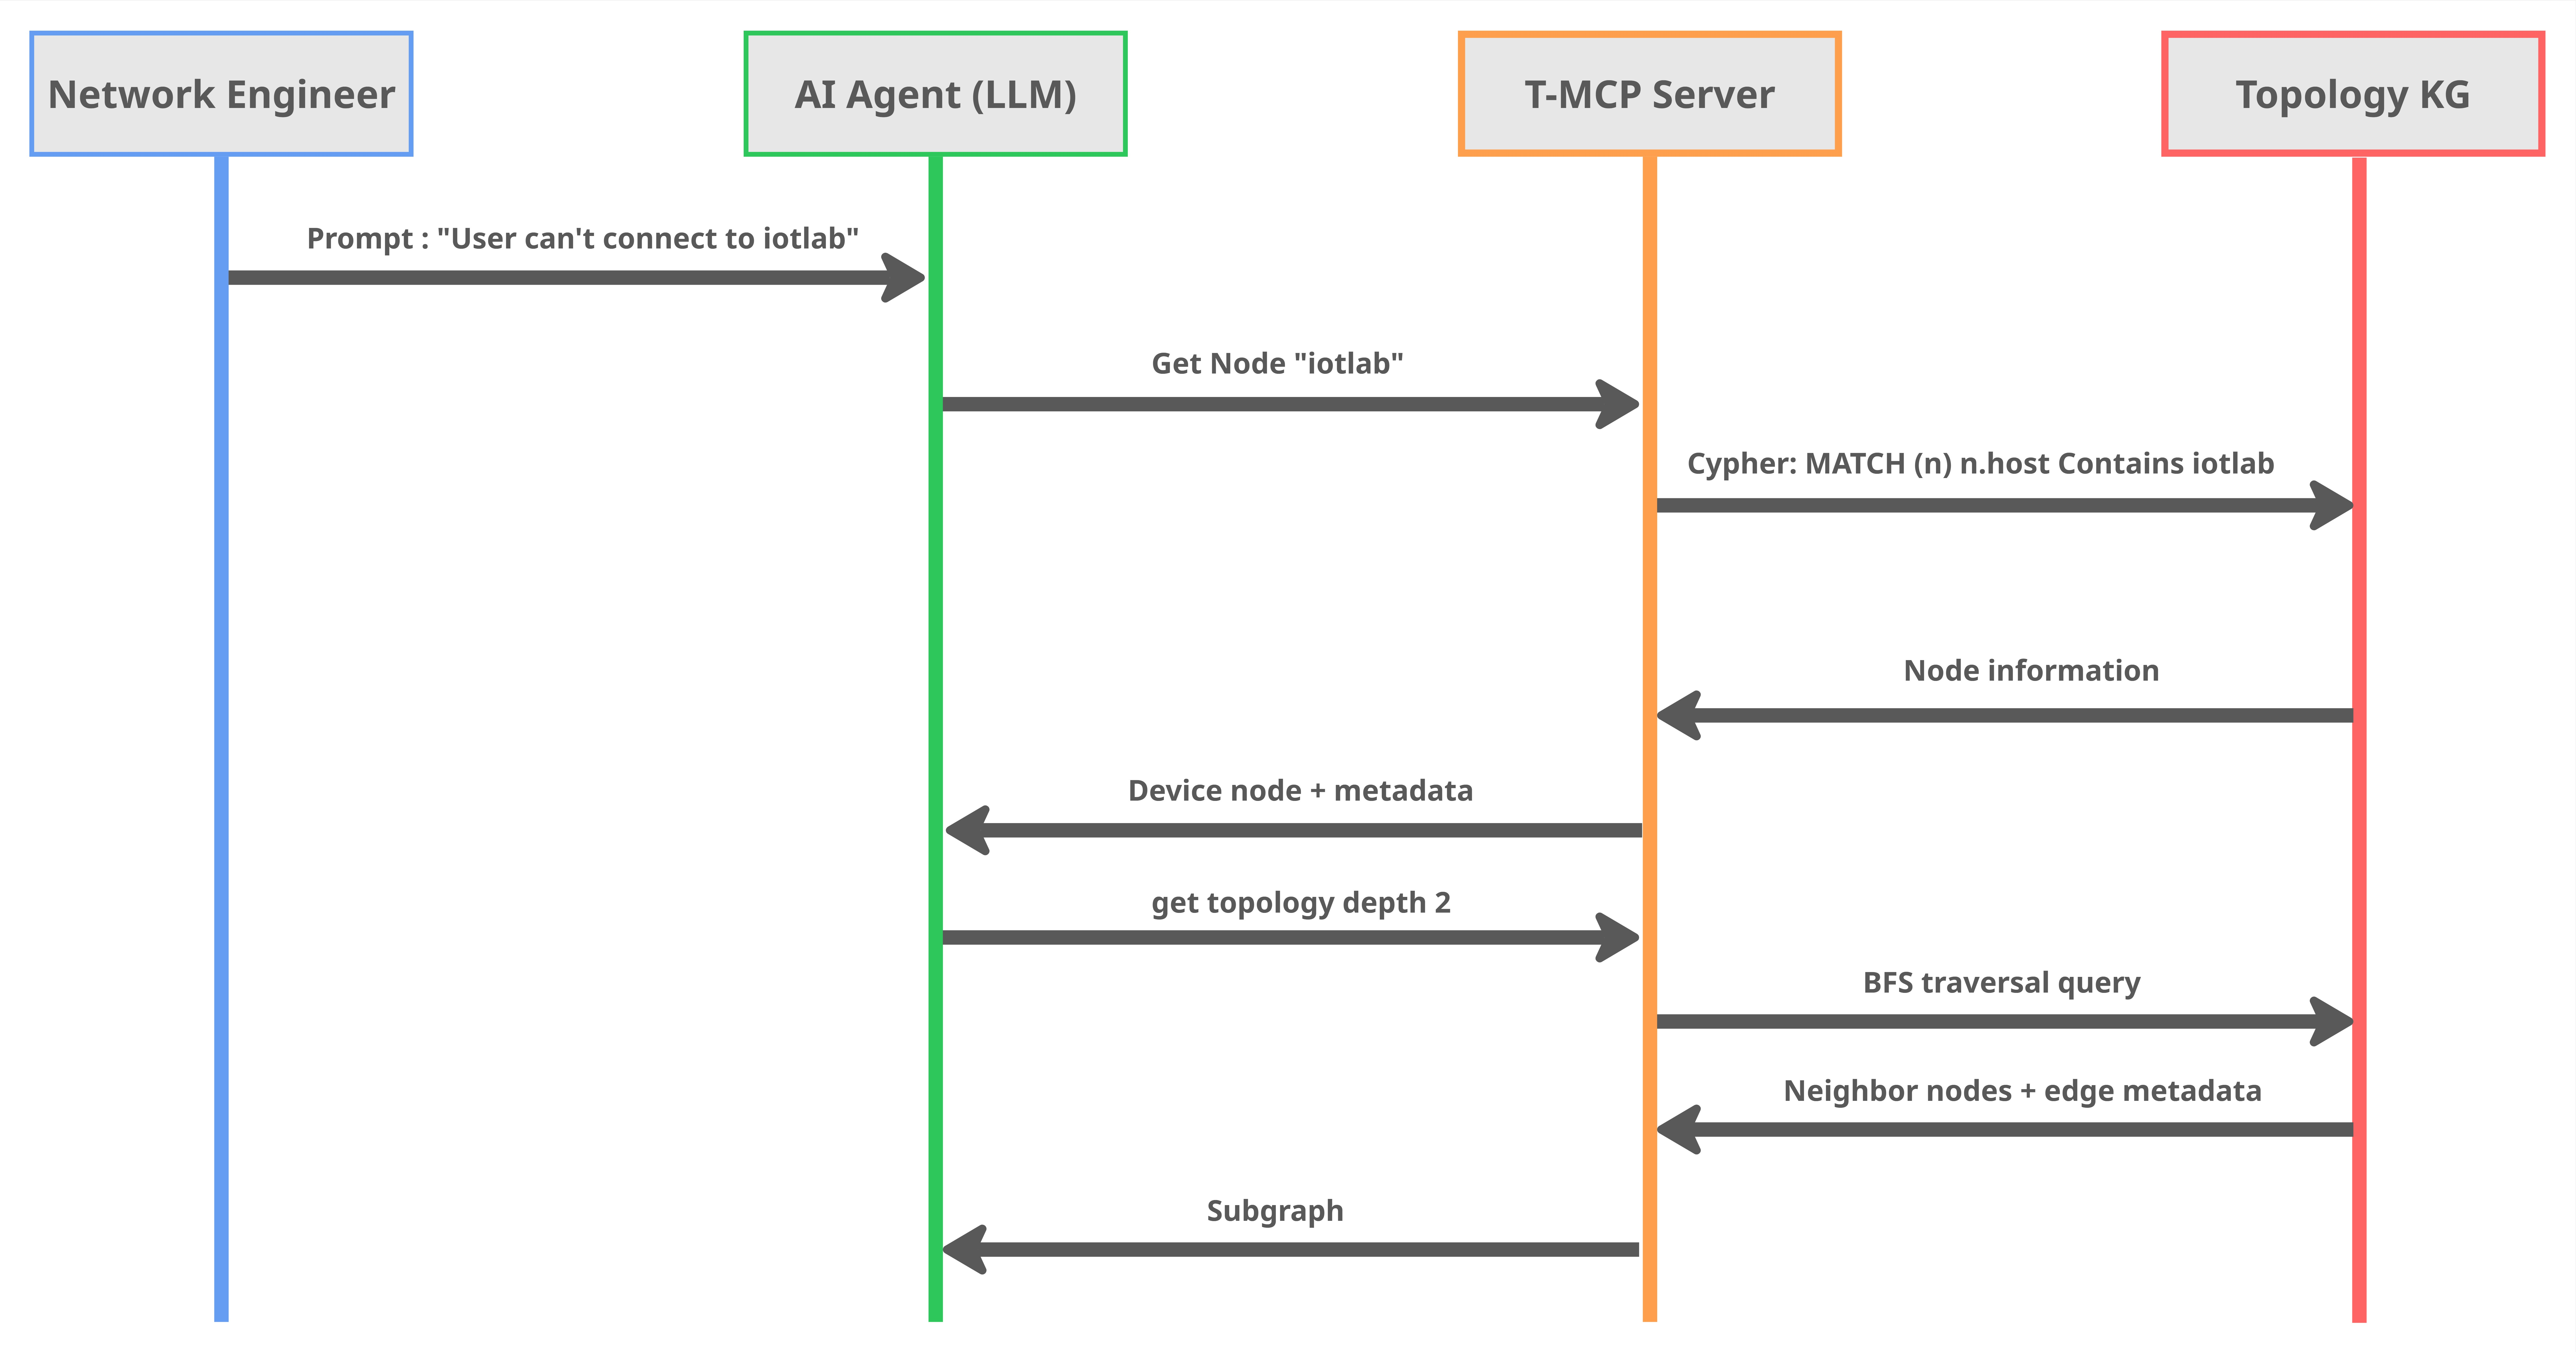
\includegraphics[width=0.85\textwidth]{images/iotlabmcp.jpg}
    \caption{ \gls{tmcp}  Dynamic interaction Sequence}
    \label{fig:iotlabmcp}
\end{figure}


Such steps involve all the activities performed by an experienced engineer in the process of fault detection and diagnosis, including \gls{fqdn} resolution, navigation of the network graph, verifying the link states, and taking remedial actions. It can be seen that  \gls{tmcp}  condition is devoid of any \gls{hallucination} regarding any topological assertions as all these facts are verified using live queries on the  \gls{neo4j}  graph.

% ─────────────────────────────────────────────────────────────────────
\section{Comparative Analysis}

Table~\ref{tab:eval} summarizes the performance of each condition 
across the three evaluation dimensions.

\begin{table}[H]
\centering
\caption{Comparative evaluation of the four conditions on the 
test fault scenario.}
\label{tab:eval}
\small
\begin{tabular}{p{3.5cm} p{2.8cm} p{2.8cm} p{3cm}}
\toprule
\textbf{Condition} & \textbf{Diagnostic Precision} & 
\textbf{Autonomy} & \textbf{\gls{hallucination} Risk} \\
\midrule
Baseline \gls{llm}           & Generic steps only      & None       & High \\[4pt]
Document  \gls{rag}           & Subnet-level awareness  & Low        & Medium \\[4pt]
 \gls{trag}  (KG-RAG)        & Device + neighbor aware & Medium     & Low \\[4pt]
 \gls{tmcp}  (MCP-KG)        & Full path resolution    & High       & Very Low \\
\bottomrule
\end{tabular}
\end{table}

These observations confirm the added value of each level of the topology-informed \gls{grounding} framework. The baseline demonstrates that the \gls{llm}  is unsuitable for performing autonomous network operations without contextual assistance. Semantic \gls{grounding} in Document  \gls{rag}  offers an improvement. however, it is incapable of replacing the importance of structural \gls{grounding}.  \gls{trag}  makes progress towards addressing the issue of topology blindness by \gls{grounding} the agent based on the connectivity information available at the time of the prompt creation. In turn,  \gls{tmcp}  builds on this by ensuring that the agent has access to the connectivity data as part of its reasoning cycle.




\chapter{Conclusion}

\section{Summary of Technical and Scientific Contributions}

This thesis is concerned with one of the primary drawbacks of using Large Language Models in managing networks: the absence of a topological understanding. Today's systems, be they natural language-based, document-based, or agent-based, operate without an understanding of the physical and logical connections within an enterprise network. Because of the lack of such a basis, \gls{ai}agents would produce erroneous configurations, misdiagnose issues, and be unable to determine how faults propagate through device dependencies.

To address this limitation, three contributions have been created and merged into a single system. The first contribution is an automated system for topology discovery and the creation of a Knowledge Graph representation. The method combines iterative polling by \gls{snmp} and \gls{lldp} -based neighbor advertisement into a recursive algorithm capable of discovering the entirety of the accessible topology starting from a seed node. The result is a living  \gls{neo4j}  graph database, where each device is represented as a node, connections between devices are edges, and device metadata are stored as properties.

The second contribution is the Topology-Aware Retrieval-Augmented Generation ( \gls{trag} ) system.  \gls{trag}  extracts candidate device identifiers from the natural language query (prompt), searches the knowledge graph across hostname,description, and location fields, and retrieves the one-hop neighbourhood of each matched device, serializing the result as a compact YANG-style context block injected into the \gls{llm}  prompt. Unlike flat document  \gls{rag} ,  \gls{trag}  preserves structural relationships and constrains the context window to only the topologically relevant neighbourhood of the queried device. While in contrast with flat documents used in existing  \gls{rag}  models,  \gls{trag}  preserves multi-hop relations and selects only topology-specific neighborhoods relevant to the queried device, ensuring that the context window remains constrained and thus minimizing \gls{hallucination}s.

The third contribution is Topology-MCP ( \gls{tmcp} ), which offers an on-demand usage of the topology knowledge graph as an \gls{mcp}  tool, callable by the \gls{ai}agent as part of its reasoning process. Thus, instead of being a passive retrieval system,  \gls{tmcp}  becomes an actively employed cognitive mechanism, where the \gls{ai}itself decides when the context is needed, performs the relevant queries based on device IDs, and automatically integrates the extracted information in reasoning. Evaluation shows that with this combination of tools, it is possible to achieve full path resolution without \gls{hallucination}, as well as autonomous recommendations for remediation features not seen before in evaluation, and impossible to obtain with other setups.

All of these contributions are combined in a single Network Operations Platform ( \gls{nop} ), a modular and containerized solution that enables uniform access for network engineers to automation and \gls{ai}diagnostic tools, a knowledge base with documentation, and a live topology graph provided by  \gls{neo4j} -db.

% ─────────────────────────────────────────────────────────────────────
\section{Potential Uses and Applicability}

The benefits of the presented thesis can be directly used in production networks. As  \gls{nop}  operates within the network infrastructure based on \gls{snmp} and \gls{lldp} , the immediate transferability of the platform is ensured in terms of the multi-vendor, multi-site WAN and LAN infrastructure used by the network operations team. Within a relatively short period, the  \gls{nop}  platform has the potential to decrease  \gls{mttr}  via providing network engineers with assistance in troubleshooting and automatic recommendations for fixing problems grounded in topology-related issues, thus avoiding manual work that includes correlation of logs, configuration files, and \gls{topology} schemes.


The proposed solution is scalable and can be implemented in any other company or service provider managing their heterogeneous network infrastructure at scale. The proposed architecture is inherently vendor agnostic since the discovery pipeline uses industry-standard protocols, and the knowledge graph structure can represent any device.

Academically speaking, the  \gls{trag}  and  \gls{tmcp}  approaches offer a reusable pattern of designing for situations where interdependence exists between elements, not limited to networking but also applicable to fields such as cloud computing, IoT, and logistics. In any field where there is a reasoning gap, just like in flat  \gls{rag} , the combination of performing a search in a knowledge graph if necessary and making use of the available \gls{mcp}  tools for reasoning purposes is a solution.
% ─────────────────────────────────────────────────────────────────────
\section{Future Perspectives}

Several directions remain open for future work. The most immediate extension is the integration of real-time telemetry ingestion into the knowledge graph. Currently, the  \gls{neo4j}  graph represents a structural snapshot of the network that is refreshed by re-running the discovery pipeline. Streaming telemetry via protocols such as gRPC or gNMI would allow the graph to reflect live interface states, traffic loads, and alarm conditions, enabling the \gls{ai}agent to reason about the network's current operational state rather than its last-known configuration.

A second direction is the development of proactive \gls{aiops} capabilities. The current platform is reactive: it responds to user-initiated queries and fault reports. Extending the agent with anomaly detection over the topology graph  identifying unusual patterns in neighbor adjacency, link utilization, or configuration drift  would enable proactive alerting before incidents escalate and are reported by users.


Finally, extending the platform to support configuration validation through integration with tools such as Batfish would close the loop between topology-aware diagnosis and verified remediation: the agent could not only identify a fault and propose a fix, but validate that the proposed configuration change is correct before execution, bringing the platform closer to the zero-touch management ideal that Intent-Based Networking has long envisioned.


% ==============================================================================
% PART II: BACK MATTER
% ==============================================================================

\bibliographystyle{IEEEtran}
\bibliography{references}

\printglossaries

\appendix
\chapter{ \gls{neo4j}  Knowledge Graph Schema}

The following table details the complete schema of the  \gls{neo4j}  
knowledge graph used by  \gls{trag}  and  \gls{tmcp} . It defines node types, 
edge types, and the properties stored on each entity.

\begin{table}[H]
\centering
\caption{ \gls{neo4j}  Knowledge Graph Schema}
\small
\begin{tabular}{p{2.5cm} p{2.5cm} p{7cm}}
\toprule
\textbf{Type} & \textbf{Label} & \textbf{Properties} \\
\midrule
Node & Device & sysid, hostname, ip\_addresses, vendor, 
                model, type, location, active\_status \\[4pt]
Edge & CONNECTED\_TO & source\_port, dest\_port, link\_speed, 
                       oper\_status \\[4pt]
Edge & PEER & protocol, session\_state \\[4pt]
Edge & MANAGED\_BY & management\_ip, \gls{snmp}\_version \\
\bottomrule
\end{tabular}
\end{table}

\chapter{Sample  \gls{tmcp}  Tool Interface}

The  \gls{tmcp}  \gls{mcp}  server exposes the following tools to the \gls{ai}agent:

\begin{table}[H]
\centering
\caption{ \gls{tmcp}  MCP Tool Definitions}
\small
\begin{tabular}{p{3cm} p{3cm} p{6cm}}
\toprule
\textbf{Tool Name} & \textbf{Input Parameters} & \textbf{Output} \\
\midrule
get\_device\_subgraph & identifier (sysid/IP/hostname), 
                        depth (int, default 1) & 
                        Serialized subgraph: device node + 
                        neighbors + edge metadata \\[4pt]
get\_neighbors & identifier & 
                 List of directly connected devices 
                 with port and link status \\[4pt]
get\_path & source, destination & 
            Shortest path between two devices 
            with all intermediate hops \\
\bottomrule
\end{tabular}
\end{table}


% ==============================================================================
% PART III: COMPANY ACTIVITY REPORT (MANDATORY STRUCTURE)
% ==============================================================================

\chapter{Company Activity Report}

\section{Presentation of the Activity}

Stellantis is mainly known as an automobile manufacturer, but from the inside it is clear that the company is also highly dependent on digital infrastructure. The activity of the company is not only about producing cars, but also about connecting many brands, factories, offices, engineering centers, suppliers, and digital services together. In a company of this size, the network becomes a critical production tool. If the network is not working, users cannot access their applications, industrial systems may be impacted, internet access can be unavailable, and in some cases production itself can be slowed down or blocked. In simple terms, for Stellantis, no network can also mean no cars, no users, and no sales.

The internship took place in a network engineering environment, more specifically within the NETS--NESA organization. This environment is responsible for designing, maintaining, and improving the network architecture used by Stellantis sites. The networks concerned are not small isolated laboratory networks, but real production infrastructures including data centers, campus networks, LAN, WAN, Wi-Fi, industrial sites, and interconnections between different geographical locations.

The activity of the team is mainly focused on architecture, design, standardization, audits, and support for operational teams. The team works on High-Level Design (HLD), Low-Level Design (LLD), global network standards, and technical decisions related to technologies such as Cisco, Aruba, Palo Alto, F5, and other enterprise networking solutions. One important lesson I learned is that even if the network is very large, it becomes easier to understand when standards are respected. The real difficulty appears when standards are not followed, when legacy constraints exist, or when some parts of the infrastructure have evolved differently over time.

Compared to an academic or laboratory environment, the main difference is the impact of every decision. In a school lab, a wrong configuration usually only affects the experiment. In a real production network, a wrong change can impact users, business applications, factories, or security. This is why the work must be structured, validated, documented, and aligned with company processes. This also explains why automation and \gls{ai}cannot be introduced as simple experiments: they must be designed to assist engineers safely, with human validation before any sensitive production action.

My internship was positioned at the intersection between networking, automation, and artificial intelligence. The objective was not only to build a chatbot, but to explore how \gls{ai}can really help network engineers in their daily work. This included reducing troubleshooting time, helping engineers find information faster, automating repetitive tasks, assisting with incident analysis, and creating tools that are useful in a real enterprise context.

\section{The Host Company}

Stellantis is a worldwide automobile manufacturer created in 2021 through the merger of PSA Group and Fiat Chrysler Automobiles. The group brings together many automotive brands and operates in several countries with factories, offices, engineering sites, data centers, and digital platforms. This scale makes the IT and network infrastructure a central part of the company activity.

The internship was carried out within the Digital \& IT environment of Stellantis, in the NETS-NESA organization. NETS is the network entity responsible for network services, while NESA is more focused on network solutions architecture. The team works on the design and evolution of network architectures used across Stellantis sites. Its role is to define technical standards, support network transformation, validate solutions, and help ensure that the infrastructure remains coherent at a global scale.

The team interacts with different technology domains and vendors, including Cisco, Aruba, Palo Alto, BT and other enterprise networking solutions. The work covers several types of networks such as LAN, WAN, Wi-Fi, data center connectivity, firewalling, and industrial network access. Because Stellantis operates at a global scale, the network environment is heterogeneous and complex. However, the use of common standards helps make this infrastructure manageable and easier to troubleshoot.

During the internship, I was integrated into this environment with a specific focus on \gls{AINetOps} and network automation. My work was exploratory and innovation-oriented, but it was also connected to real operational needs. The objective was to build solutions that could support engineers in practical tasks, not only demonstrate \gls{ai}concepts in isolation.

\section{The Internship Supervisor}

My company supervisor was Jérémy Chassignol, a network architect at Stellantis. He has long experience in enterprise networking and has worked on the evolution of network architectures from PSA Group to Stellantis. His role involves defining and maintaining network architecture standards used across the company, especially for LAN and WAN environments.

Jérémy supported me throughout the internship by giving me both technical guidance and autonomy. He helped me understand the reality of large enterprise networks, the importance of standards, and the constraints that exist in production environments. At the same time, he allowed me to explore new ideas, test technical approaches, and make architectural decisions for the \gls{AINetOps} platform.

I also worked in an environment supported by Khaled Hammami and Nicolas Decre, who helped create the conditions for my internship and gave me the opportunity to work on innovative topics related to artificial intelligence and network operations. This context was important because the subject required both technical freedom and alignment with real company needs.

\section{Summary of Proposed Work}

The main direction of my internship was to explore how artificial intelligence and automation can improve network operations inside Stellantis. The central result of this work was the development of a Network Operations Platform, called  \gls{nop}  in this report. The goal of  \gls{nop}  was to provide network engineers with a platform where they can ask questions, search documentation, diagnose incidents, query topology, launch automation scripts, and use AI-assisted workflows.

The platform was designed to assist engineers, not replace them. This was an important principle from the beginning. In networking, an incorrect action can have serious consequences, so the \gls{ai}must be grounded in reliable data and sensitive actions must remain under human validation. For this reason, the platform does not blindly execute changes in production. It provides assistance, proposes actions, and allows validation before execution.

Several workstreams were developed during the internship for the  \gls{nop} :

\begin{itemize}
    \item the design and implementation of the  \gls{nop}  platform
    \item the integration of \gls{ai}agents for network operations
    \item the connection of the agent to documentation through  \gls{rag} 
    \item the automatic discovery of \gls{topology} using \gls{\gls{snmp}} and \gls{lldp} 
    \item the construction of a  \gls{neo4j}  knowledge graph representing network devices and links
    \item the implementation of topology-aware \gls{ai}mechanisms such as  \gls{trag}  and  \gls{tmcp} 
    \item the integration of automation scripts such as DNS lookup, ping, SSH checks, and diagnostic tools
    \item the connection to ServiceNow incident information through an \gls{mcp}  server
    \item the automation of IoT device onboarding and homologation workflows
    \item the demonstration of \gls{ai}usage in different network engineering and operations workflows.
\end{itemize}

The first project I worked on was related to the automation of new IoT device onboarding. Before this work, the process was mainly based on Excel files. A requester filled an Excel sheet, then the network and security teams reviewed the requested flows, and firewall rules were created manually. This process could take several iterations because the requester might forget some flows, which would block the IoT device during testing.

The new approach aimed to make this process more automatic and more reliable. The platform registers the device, assigns a static IP address using Infoblox, registers the MAC address in Cisco ISE, connects the device to a dedicated Wi-Fi environment, captures traffic flows, analyzes them using Zeek, generates firewall rules, sends them for validation by the security team, and finally pushes the approved rules to Palo Alto firewalls through \gls{api} calls. The main benefit of this work was to reduce a process that could take weeks into a process that can be completed in days.





In parallel, I worked on  \gls{nop}  as a broader \gls{AINetOps} platform. This platform was built using technologies such as Python, FastAPI, Docker Compose,  \gls{neo4j} , SQLite, and internal access to Claude Sonnet through a company \gls{api}. The platform also included a web interface, allowing users to interact with \gls{ai}agents, consult documentation, launch tools, and visualize topology information.



\section{Work Completed in the Company}

During the internship, I completed several technical contributions in the company. The work was not limited to one script or one prototype, but covered several parts of an AI-assisted network operations platform.

\subsection{Development of the  \gls{nop}  Platform}

The main technical work was the design and implementation of the  \gls{nop}  platform.  \gls{nop}  is a web platform created to help network engineers interact with documentation, automation tools, topology information, and \gls{ai}agents from one place. The platform allows engineers to ask network-related questions, retrieve relevant documents, analyze incidents, query \gls{topology}, and launch diagnostic scripts.

The platform was built with a modular architecture. The backend was developed mainly in Python using FastAPI. Docker Compose was used for deployment, which made it easier to run the different services together. SQLite was used for some platform data, while  \gls{neo4j}  was used for the topology knowledge graph. The \gls{ai}part used Claude Sonnet through an internal \gls{api}. The platform was designed as a pre-production solution, with the objective of moving progressively toward production after validation.

The platform also included a web interface, so the work was not only backend-oriented. The interface allowed users to access AI-assisted tasks, view information, and interact with network automation functions. This was important because the objective was to make something usable by engineers, not only a technical demonstration.

\begin{figure}[H]
    \centering
    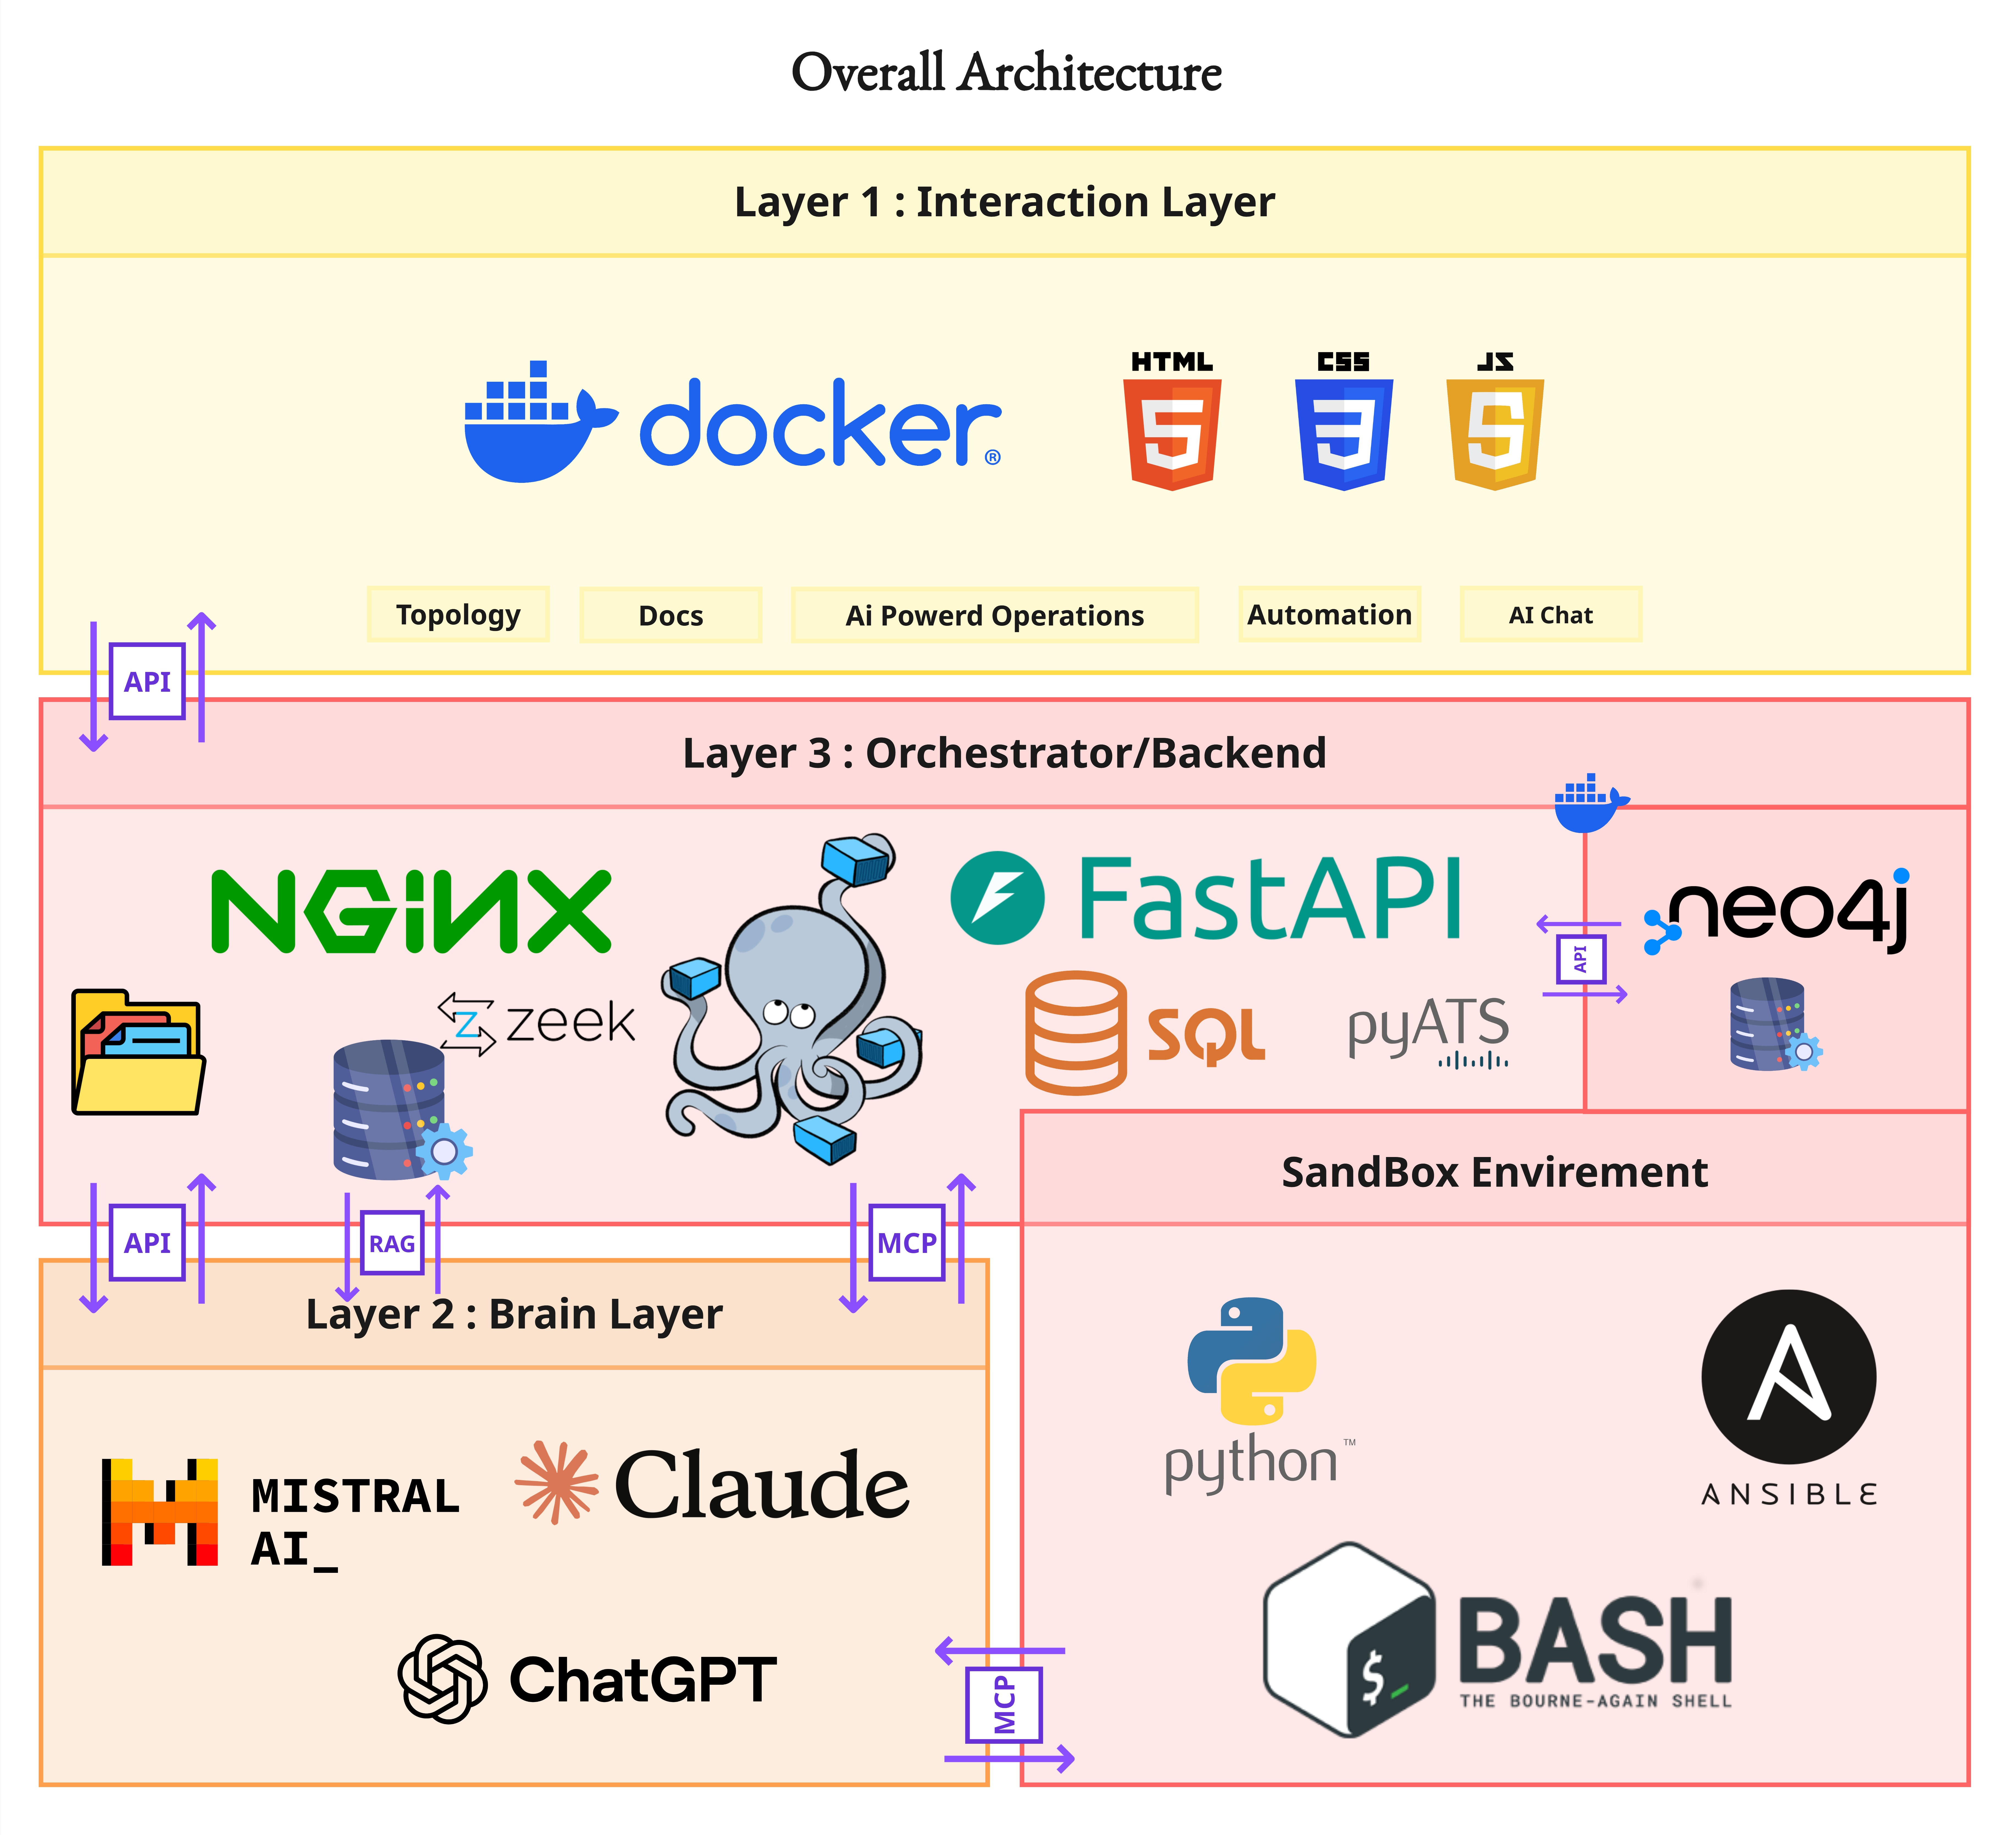
\includegraphics[width=0.85\textwidth]{images/nop.jpg}
    \caption{ \gls{nop}  Overall Architecture}
    \label{fig:NOP}
\end{figure}


\subsubsection{AI Agent for Network Operations}

A major part of the work was the creation of an \gls{ai}agent dedicated to network operations. The agent could answer technical questions, search internal documentation, query the topology graph, analyze incidents, suggest remediation steps, and execute automation scripts when approved by a human.

The agent was connected to different sources of information. First, document  \gls{rag}  was used to search network standards, HLD and LLD documents, operational procedures, and architecture documents. This allowed the agent to answer questions using company-specific knowledge instead of relying only on general model knowledge.

Second, the agent was connected to topology information through the  \gls{trag}  and  \gls{tmcp}  mechanisms described in the technical part of this thesis.  \gls{trag}  allowed the agent to receive relevant topology context before answering, while  \gls{tmcp}  allowed it to dynamically query the topology graph during its reasoning process. This was one of the most important aspects of the work because it helped reduce \gls{hallucination}s and made the \gls{ai}more useful for real troubleshooting.

The agent could also launch automation scripts such as DNS lookup, ping, SSH checks, and other diagnostic tools. However, execution was controlled with human validation, especially when the action could affect production. This design choice was important because the goal was to assist network engineers while keeping control and safety.


\begin{figure}[H]
    \centering
    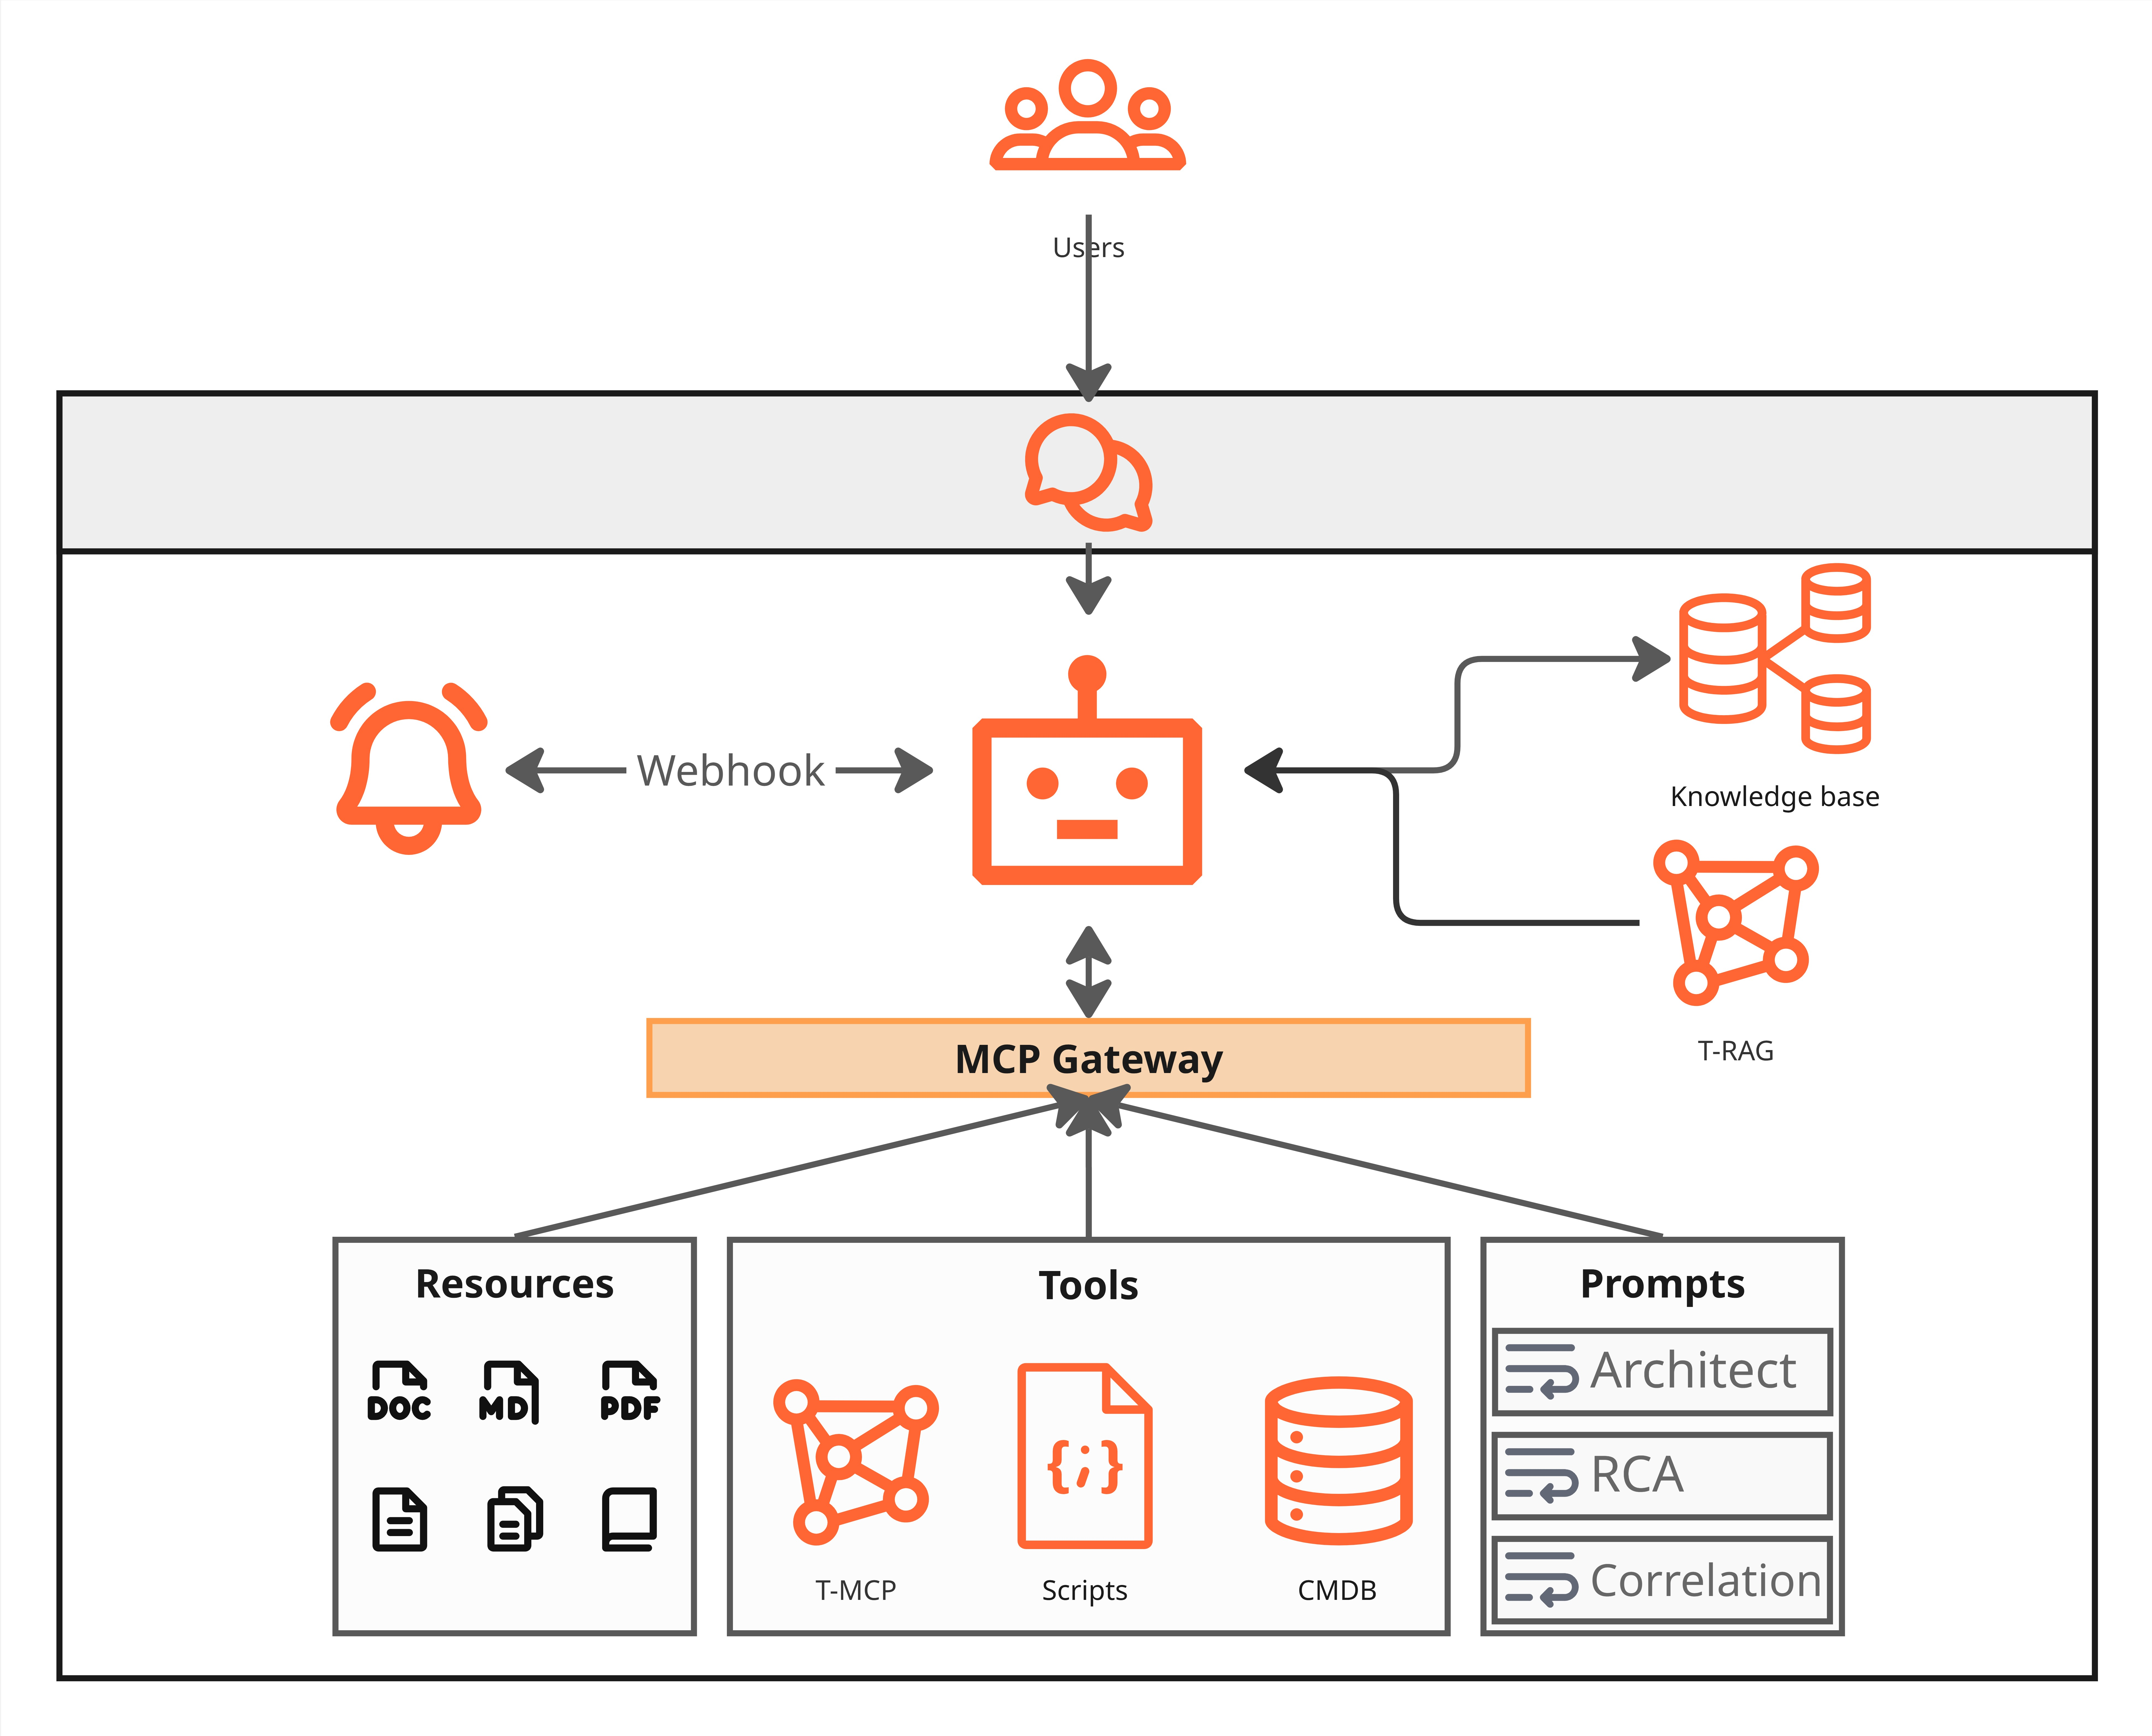
\includegraphics[width=0.85\textwidth]{images/nopoverall.jpg}
    \caption{NOP \gls{ai}Agent}
    \label{fig:NOPai}
\end{figure}


\subsection{Topology Discovery and Knowledge Graph}

Another important contribution was the automatic topology discovery system. The objective was to discover network devices and their connections using \gls{\gls{snmp}} and \gls{lldp} , then store this information in  \gls{neo4j}  as a knowledge graph.

The topology discovery was tested on real production network environments. This made the work more realistic but also more difficult. Some devices had \gls{\gls{snmp}} or \gls{lldp}  disabled, and in some cases information was incomplete. This showed the difference between a clean lab environment and a production environment. In production, discovery depends on access rights, device configuration, security constraints, and the quality of the information exposed by the equipment.

The topology graph was useful because it allowed engineers and \gls{ai}agents to understand where a device is connected, identify the upstream switch, trace a path, understand dependencies, and troubleshoot faster. In addition to graph queries, topology visualizations were integrated into the  \gls{nop}  platform, making the information easier to understand visually.

\begin{figure}[H]
    \centering
    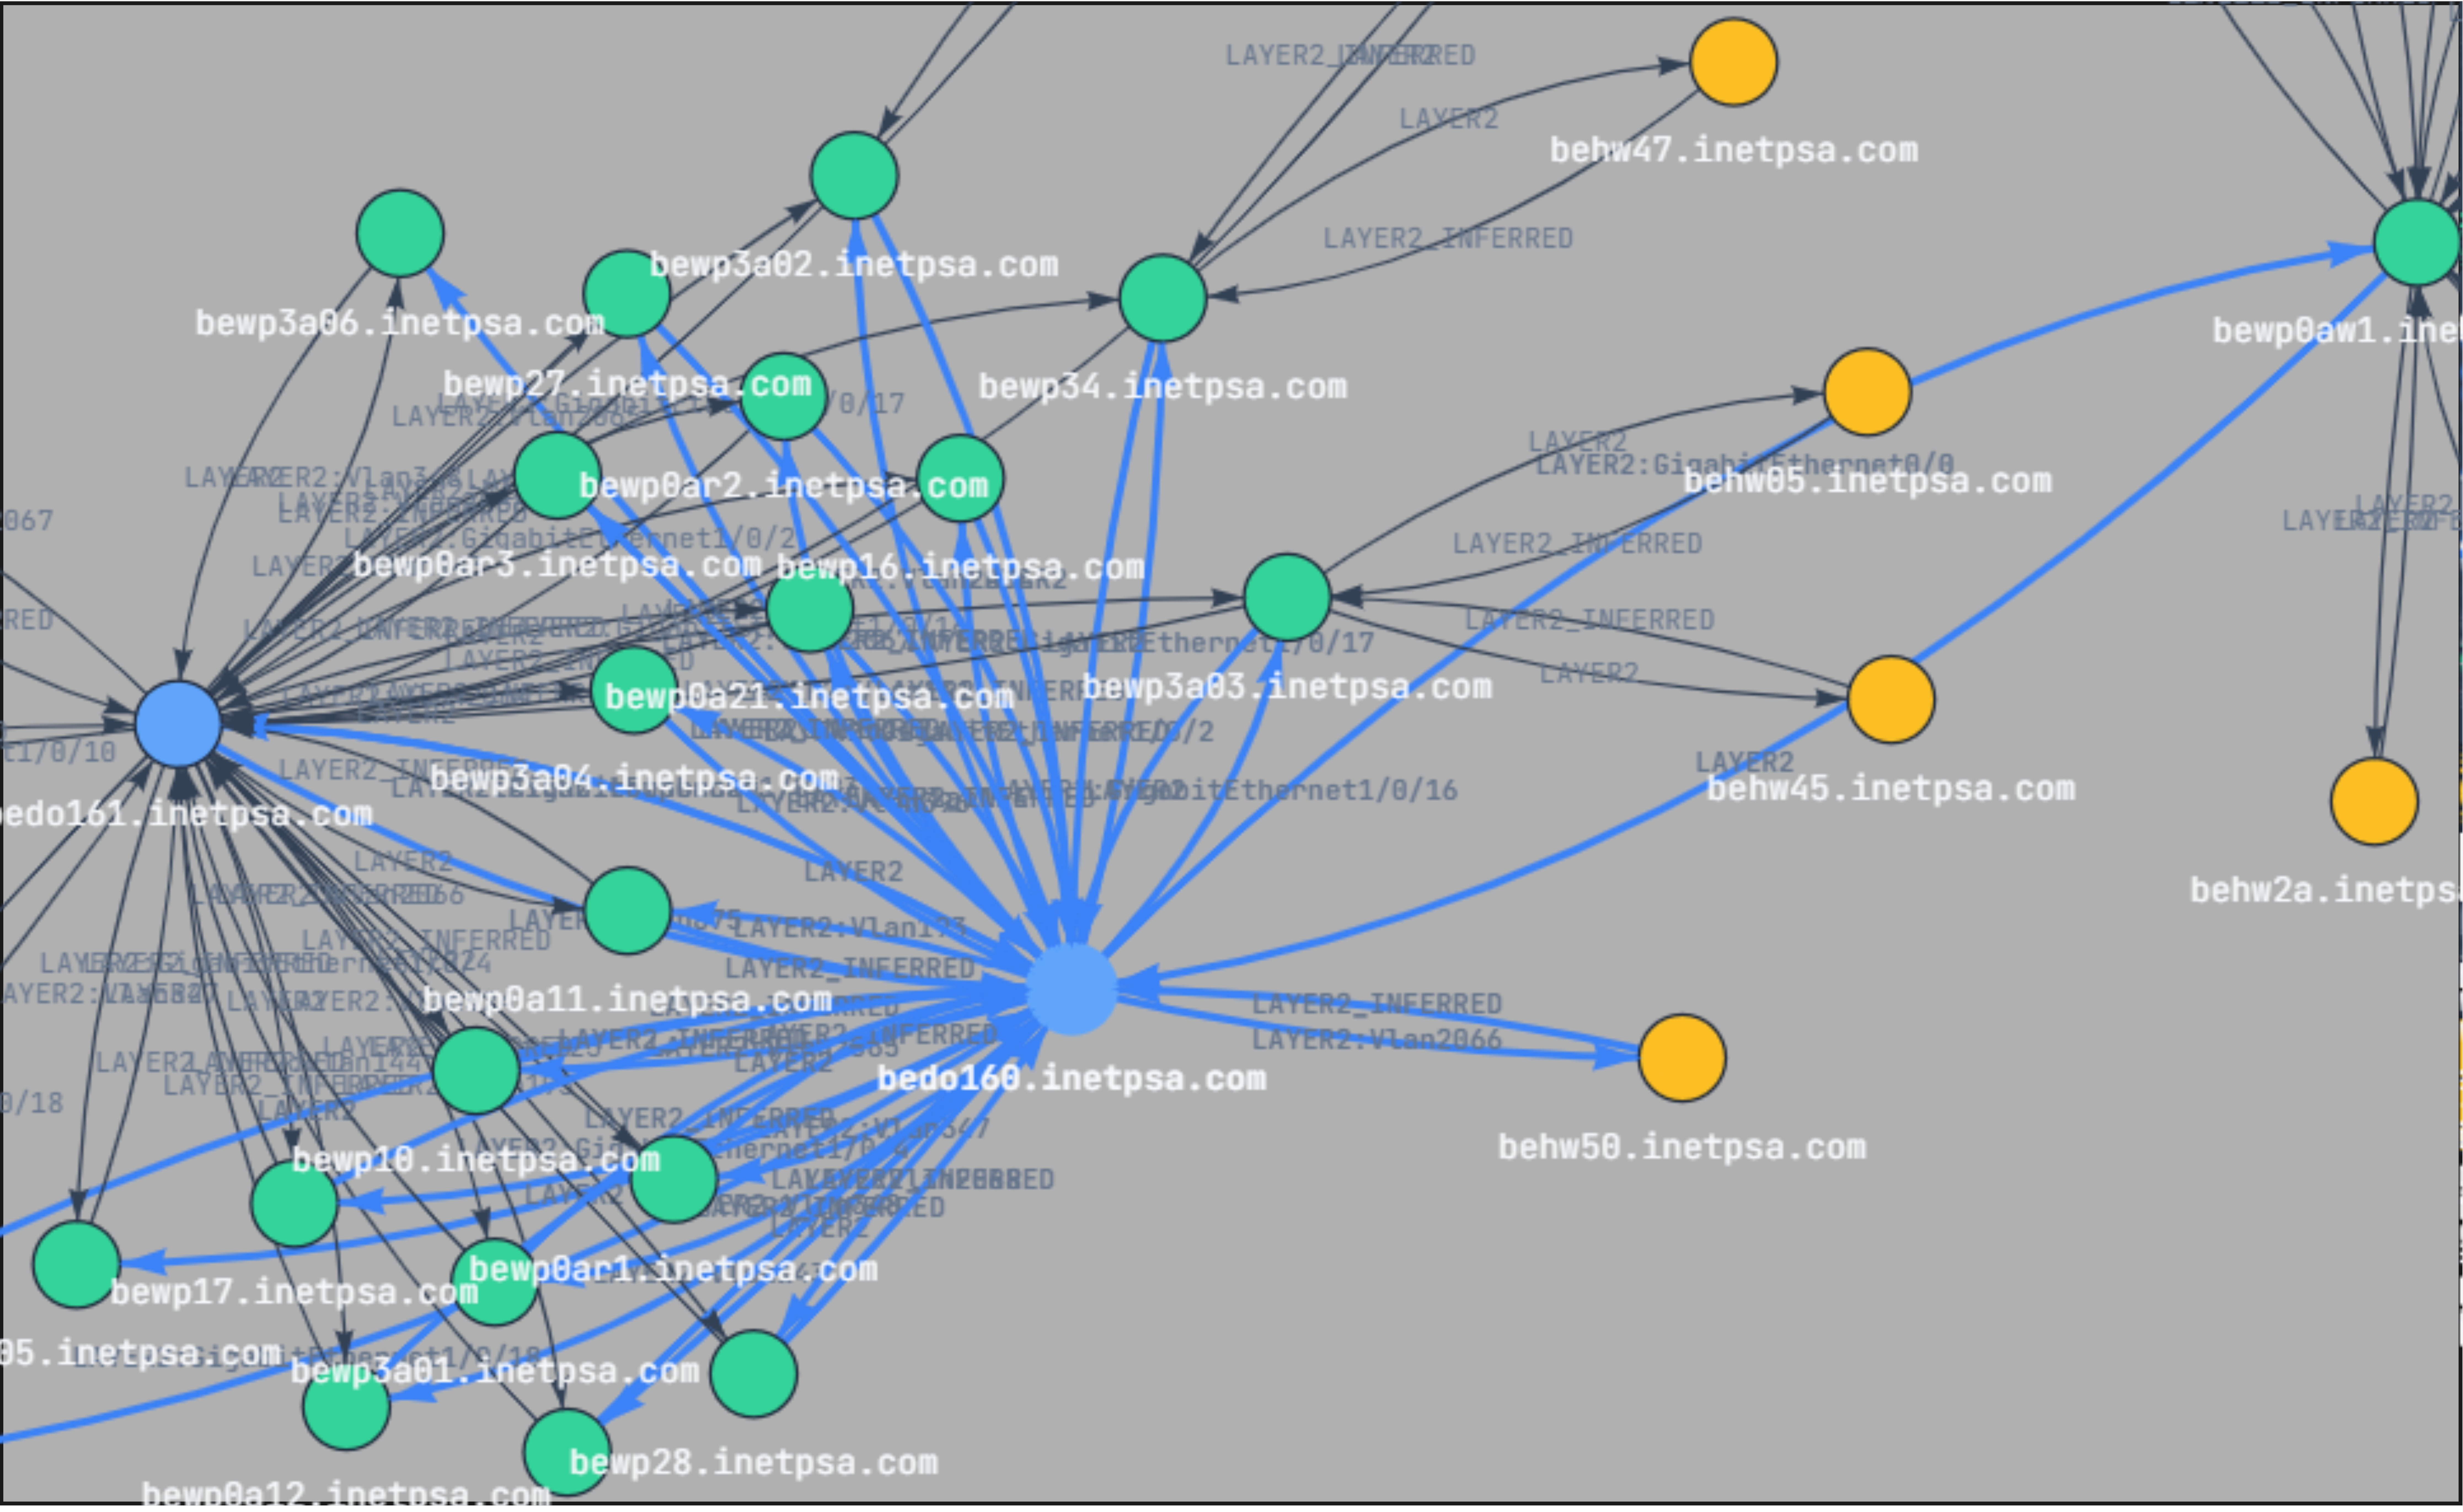
\includegraphics[width=0.85\textwidth]{images/scriptexample.jpg}
    \caption{Topology Discovery Visualization}
    \label{fig:Visualization}
\end{figure}


\subsection{IoT Device Onboarding and Homologation Automation}

The first project of the internship was focused on automating the onboarding and homologation of IoT devices. This was a very concrete company problem. The previous process relied on Excel files and manual exchanges between requesters, network teams, and security teams. If some flows were missing from the request, the IoT device could be blocked, and the process required new iterations.

The proposed workflow automated several steps. First, the device is registered using its name and MAC address. Then a static IP address is assigned through Infoblox, and the MAC address is registered in Cisco ISE. The device is connected to a dedicated Wi-Fi environment in a specific VRF with controlled internet access during homologation. Traffic is captured using PCAP files, then analyzed with Zeek to extract the flows actually used by the device. Based on this analysis, firewall rules are generated and sent to the security team for validation. After validation by the CISO/security team, the rules can be pushed to Palo Alto firewalls through \gls{api} calls.

\begin{figure}[H]
    \centering
    
\includegraphics[width=0.85\textwidth]{images/IOTautomation.jpg}
    \caption{Iot On-boarding automation workflow}
    \label{fig:iotautomation}
\end{figure}

This work was useful because it transformed a manual and iterative process into a more structured and automated workflow. The main expected gain is time reduction, moving from a process that can take weeks to a process that can be completed in days, while also improving traceability and reducing the risk of missing flows.


\subsection{ServiceNow Incident Integration}

Another part of the work concerned the integration of ServiceNow incident information into the \gls{ai}workflow. The connection was done through an \gls{mcp}  server that allowed the agent to retrieve network incident details. The goal was to help engineers save time when investigating existing incidents or looking for recent related cases.

The ServiceNow data used in this context concerned network incidents. For example, the agent could be asked to search for the last ten incidents and retrieve their details. This kind of integration is useful because network engineers often need to check whether a problem is isolated or already reported somewhere else. Giving the \gls{ai}agent access to this information makes the investigation faster and more centralized.

\subsection{AI Integration in Engineering Workflows}

Beyond the specific  \gls{nop}  and IoT projects, I also helped explore how \gls{ai}can be integrated into different workflows used by network architects and operations teams. This included documentation search, incident analysis, network design assistance, and network operations support, i was also the lead \gls{ai}community for my team where i maintain a teams channel where we exchange \gls{ai}prompts and use cases. 

I showed the platform and collected feedback from people in the team. The feedback was positive, especially because the work was not only theoretical. The platform showed concrete examples of how \gls{ai}can help engineers by reducing repetitive work, finding information faster, and improving the troubleshooting process. One of the things I am proud of is that the demos were well received and that the platform was considered close enough to continue toward production work.

\section{Conclusion of the Activity Report}

This internship allowed me to work on a subject that combines several important areas: enterprise networking, automation, artificial intelligence, and operational tooling. The company environment was very different from an academic lab because the infrastructure is real, large, heterogeneous, and constrained by security and production requirements. This made the work more difficult, but also much more valuable.

The main result of the internship was the creation of a pre-production \gls{AINetOps} platform that can assist network engineers in several tasks: documentation search, troubleshooting, topology exploration, automation script execution, incident analysis, and IoT on-boarding automation. The work also showed that \gls{ai}can be useful in network operations if it is connected to reliable data sources and if human validation remains part of the process.

The most important challenge was not only to make the technology work, but to make it useful for real engineers. A simple \gls{ai}demo is not enough in a production environment. The platform needed to respect operational constraints, integrate with existing systems, and provide practical value. This is why the work included not only \gls{ai}reasoning, but also topology \gls{grounding}, automation tools, validation workflows, and integration with company processes.

From a personal point of view, this internship helped me gain autonomy and confidence. I worked on complex topics, interacted with experienced network architects, and learned how large-scale enterprise networks are designed and operated. I also learned that \gls{ai}should not be seen as a replacement for engineers, but as a tool that can support them by reducing repetitive work, improving visibility, and accelerating diagnosis.

Overall, the company activity gave a clear industrial context to the technical work presented in this thesis. Stellantis depends strongly on its network infrastructure, and the NETS--NESA environment plays an important role in keeping this infrastructure coherent, secure, and evolutive. My contribution was to explore how \gls{ai}and automation can support this activity in a practical and safe way.




% ==============================================================================
% PART IV: GENERAL SYNTHESIS
% ==============================================================================

\chapter*{General Synthesis}
\addcontentsline{toc}{chapter}{General Synthesis}

\section*{Professional and Technical Growth}

During this internship and the process of writing this thesis, I had the opportunity to strengthen both my technical skills and my professional maturity. My internship within the NETS NESA team started on 16/02/2026 and lasted five months at the time of writing this report. The internship took place in the ICT department at Stellantis and allowed me to work in a real industrial environment, with production constraints and operational expectations.

Before starting this internship, I already had a solid background in networking thanks to my Master 1 and Master 2 projects in computer and network systems. I had also gained practical experience in \gls{api}s and Python automation during my previous internship at the data center of Evry. In addition, my academic background in intelligent systems and \gls{ai}projects had already introduced me to concepts such as Large Language Models,  \gls{rag} , and machine learning. However, this internship gave me the opportunity to apply these skills in a much more complex and realistic context.

One of the most important technical lessons was understanding the complexity of enterprise network architectures. In academic projects, network environments are often simplified and controlled. At Stellantis, I was exposed to heterogeneous infrastructures, production sites, vendor-specific constraints, and operational limitations. This helped me understand that building a useful automation solution is not only about making a script work, but also about designing something robust enough to handle real-world variability.

A major part of my work concerned network discovery and topology representation. I developed a recursive discovery mechanism based on \gls{\gls{snmp}} and \gls{lldp}  in order to collect information from real production sites. This work helped me move from a mostly theoretical understanding of \gls{\gls{snmp}} to a practical use of management information,  \gls{oid} s, \gls{lldp}  neighbors, device metadata, and connectivity information. The discovery was naturally limited to reachable equipment and devices where \gls{\gls{snmp}} was enabled, but it still provided a concrete basis for building a topology knowledge graph.

Another important technical contribution was the construction of the  \gls{neo4j}  knowledge graph. Before this internship, I had experience with relational and document-oriented databases such as SQL and MongoDB, but  \gls{neo4j}  and graph databases were new to me. I learned how to model network devices as nodes, connections as relationships, and metadata as properties. I also wrote  \gls{cypher}  queries for one-hop and multi-hop neighborhood retrieval, shortest-path computation, and searches based on hostnames, IP addresses, and locations. This experience helped me understand why graph databases are particularly relevant for \gls{topology} problems, where relationships between entities are as important as the entities themselves.

The internship also allowed me to deepen my knowledge of \gls{ai}applied to network operations. I designed and implemented the  \gls{trag}  pipeline, which retrieves relevant topology information from the knowledge graph and injects it into the \gls{llm}  context. I also implemented the  \gls{tmcp}  mechanism, exposing topology tools to the \gls{ai}agent so that it could dynamically query the graph during its reasoning process. The agent was connected not only to retrieved documentation, but also to scripts, tools, and \gls{mcp}  components. The \gls{llm}  was accessed through an internal \gls{api} using an Anthropic Sonnet model.

Through this work, I learned that building an \gls{ai}agent for network operations is very different from building a simple chatbot. The main difficulty is not only generating good natural language answers, but \gls{grounding} the model in reliable operational data. In networking, incorrect assumptions can lead to wrong diagnoses or risky actions. For this reason, the platform was designed to combine documentation, topology knowledge, automation scripts, and human validation before remediation actions.

\section*{Personal Development}

Beyond the technical aspects, this internship had a strong impact on my personal and professional development. It was my first experience working in a multinational company of this scale. Stellantis operates across many countries, and even though most of my daily work was within the NETS NESA environment, I also had the opportunity to interact with partners and understand how network architecture decisions can affect a large international organization.

I also learned how to communicate technical ideas in a professional setting. Explaining an AI-based network automation platform requires adapting the level of detail depending on the audience. Some discussions focused on architecture and network constraints, while others required explaining the value of \gls{ai}\gls{grounding}, topology discovery, or incident automation in a clear and practical way. This helped me improve my ability to present technical work in a structured and understandable manner.

The support of my supervisor, Jérémy Chassignol, was especially important throughout the internship. He gave me a high level of autonomy while still helping me stay aligned with operational needs and company constraints. This balance between independence and guidance allowed me to make architectural decisions, explore different technical solutions, and learn from practical limitations. It also helped me gain confidence in my ability to manage a complex engineering project.

This autonomy was one of the most valuable aspects of the internship. Unlike many academic assignments, where the objectives and boundaries are clearly defined, this work required me to deal with uncertainty. I had to investigate the problem, identify realistic solutions, test different approaches, and adapt the design when limitations appeared. For example, the use of  \gls{tmcp}  was motivated by the need to give the agent more dynamic access to topology information during reasoning, complementing the more static context provided by  \gls{trag} . This experience helped me develop a more mature engineering mindset.

\section*{Academic Knowledge Applied to an Industrial Context}

This internship also showed me how academic knowledge can be transferred to an industrial environment. Courses in network protocols, distributed systems, machine learning, natural language processing, and information retrieval provided a useful foundation for the work carried out during the internship. Concepts such as protocol behavior, system architecture, \gls{retrieval}s, and \gls{ai}model \gls{grounding} were directly relevant to the design of the  \gls{nop}  platform.

At the same time, the internship helped me understand the difference between academic exercises and industrial reality. In university projects, the environment is usually more controlled: datasets are often cleaner, requirements are more explicit, and evaluation is easier to define. In an industrial context, the situation is more nuanced. Equipment may come from different vendors, legacy constraints must be respected, access rights may be limited, and some parts of the infrastructure cannot be modified freely. Designing a solution in this context requires not only technical knowledge, but also pragmatism.

Writing this thesis was also an important learning experience. It was more difficult than the implementation work itself, because it required organizing several months of research and development into a coherent scientific and technical narrative. I had to explain the motivation of the work, position it in relation to existing research, describe the architecture, present the evaluation, and discuss the limitations honestly. This process helped me improve my scientific communication skills and gave me a better understanding of how to present engineering work in an academic format.

\section*{Achievement of Objectives and Self-Assessment}

The main objective of the internship was not limited to incident diagnostics, but more broadly to automating different network operations using \gls{ai}and network automation techniques. From this perspective, the  \gls{nop}  platform represents a significant outcome of the internship. The platform brings together several components: documentation retrieval, topology discovery, a  \gls{neo4j}  knowledge graph,  \gls{trag} ,  \gls{tmcp} , automation scripts, and an \gls{ai}agent capable of assisting network engineers.

The platform has been created and demonstrated, although it still requires additional work before a full production deployment. In particular, production integration would require further validation, security review, operational monitoring, and adaptation to company processes. However, the results obtained in the lab and through realistic scenarios show that the approach is promising.

The evaluation presented in this thesis was based on real experiments, demonstrations, screenshots, and manual comparison between several configurations: a baseline \gls{llm} , document-based  \gls{rag} ,  \gls{trag} , and  \gls{tmcp} . The results showed that topology-aware \gls{grounding} improves the relevance of the agent's reasoning. In particular,  \gls{tmcp}  allowed the agent to retrieve topology dynamically, identify the relevant path, and support troubleshooting more effectively than approaches relying only on general knowledge or static documentation.

However, the results should be interpreted carefully. \gls{hallucination} reduction was observed qualitatively rather than measured through a formal quantitative benchmark. Similarly, the remediation process was not designed as an uncontrolled fully autonomous action. In the tested scenario, the agent could use an SSH-based script to fix the issue, but the action was performed with human validation. This is an important point because network automation must remain safe, auditable, and controlled, especially in production environments.

Overall, I consider the internship successful because it allowed me to build a concrete platform, validate the relevance of topology-aware \gls{ai}for network operations, and identify the remaining work required for production use. It also helped me understand the importance of designing \gls{ai}systems that assist engineers instead of replacing their judgment.

\section*{Future Perspectives and Career Outlook}

This internship confirmed my interest in the intersection between artificial intelligence and network operations. The field of \gls{AINetOps} is particularly motivating for me because it combines several areas that I enjoy: networking, automation, and intelligent systems. As enterprise networks become more complex, I believe that AI-assisted tools will become increasingly important for helping engineers diagnose incidents, understand dependencies, and automate repetitive tasks safely.

Several future improvements could be made to the platform. One important direction would be to integrate more real-time telemetry into the knowledge graph, so that the \gls{ai}agent can reason not only on topology but also on live operational states such as interface status, alarms, traffic levels, and configuration changes. Another possible direction would be to strengthen validation mechanisms before remediation, for example by integrating configuration verification tools or approval workflows.

From a professional point of view, this internship helped me clarify that I would like to continue working in \gls{AINetOps} or related areas such as network automation, \gls{aiops}, platform engineering, or \gls{ai}infrastructure. I am still open regarding the exact path I will follow, whether in industry or possibly later in research, but I am confident that the combination of \gls{ai}and network systems is a direction in which I want to continue developing my skills.

In conclusion, this internship was a very valuable experience both technically and personally. It allowed me to apply my academic knowledge to real operational challenges, discover the complexity of large-scale enterprise networks, and contribute to the development of an AI-powered network operations platform. It also helped me grow as an engineer by learning how to work with autonomy, communicate technical ideas, and design solutions that remain realistic in an industrial environment.
\end{document}